\section{使用方法}

本研究のシステムの使用方法を述べる.使用手順は以下の通りである.

\begin{quote}
  \begin{enumerate}
    \item アプリを起動する
    \item 旅程パッケージを作成する
    \item 旅程データを作成する
    \item 通知を受け取る
    \item 災害注意予報を確認する
    \item ストック情報を確認する
  \end{enumerate}
\end{quote}

\subsection{アプリを起動する}
アプリを利用するのに,旅行計画の作成が必要であるため,機能メニューの旅行計画をタップする.
ホーム画面はアプリを立ち上げたとき,最初に表示される画面である.
この画面ではアプリの概要について説明が閲覧できる.
この画面から予報についての画面と旅程パッケージの作成画面に遷移できる.

\begin{figure}[H]
  \centering
  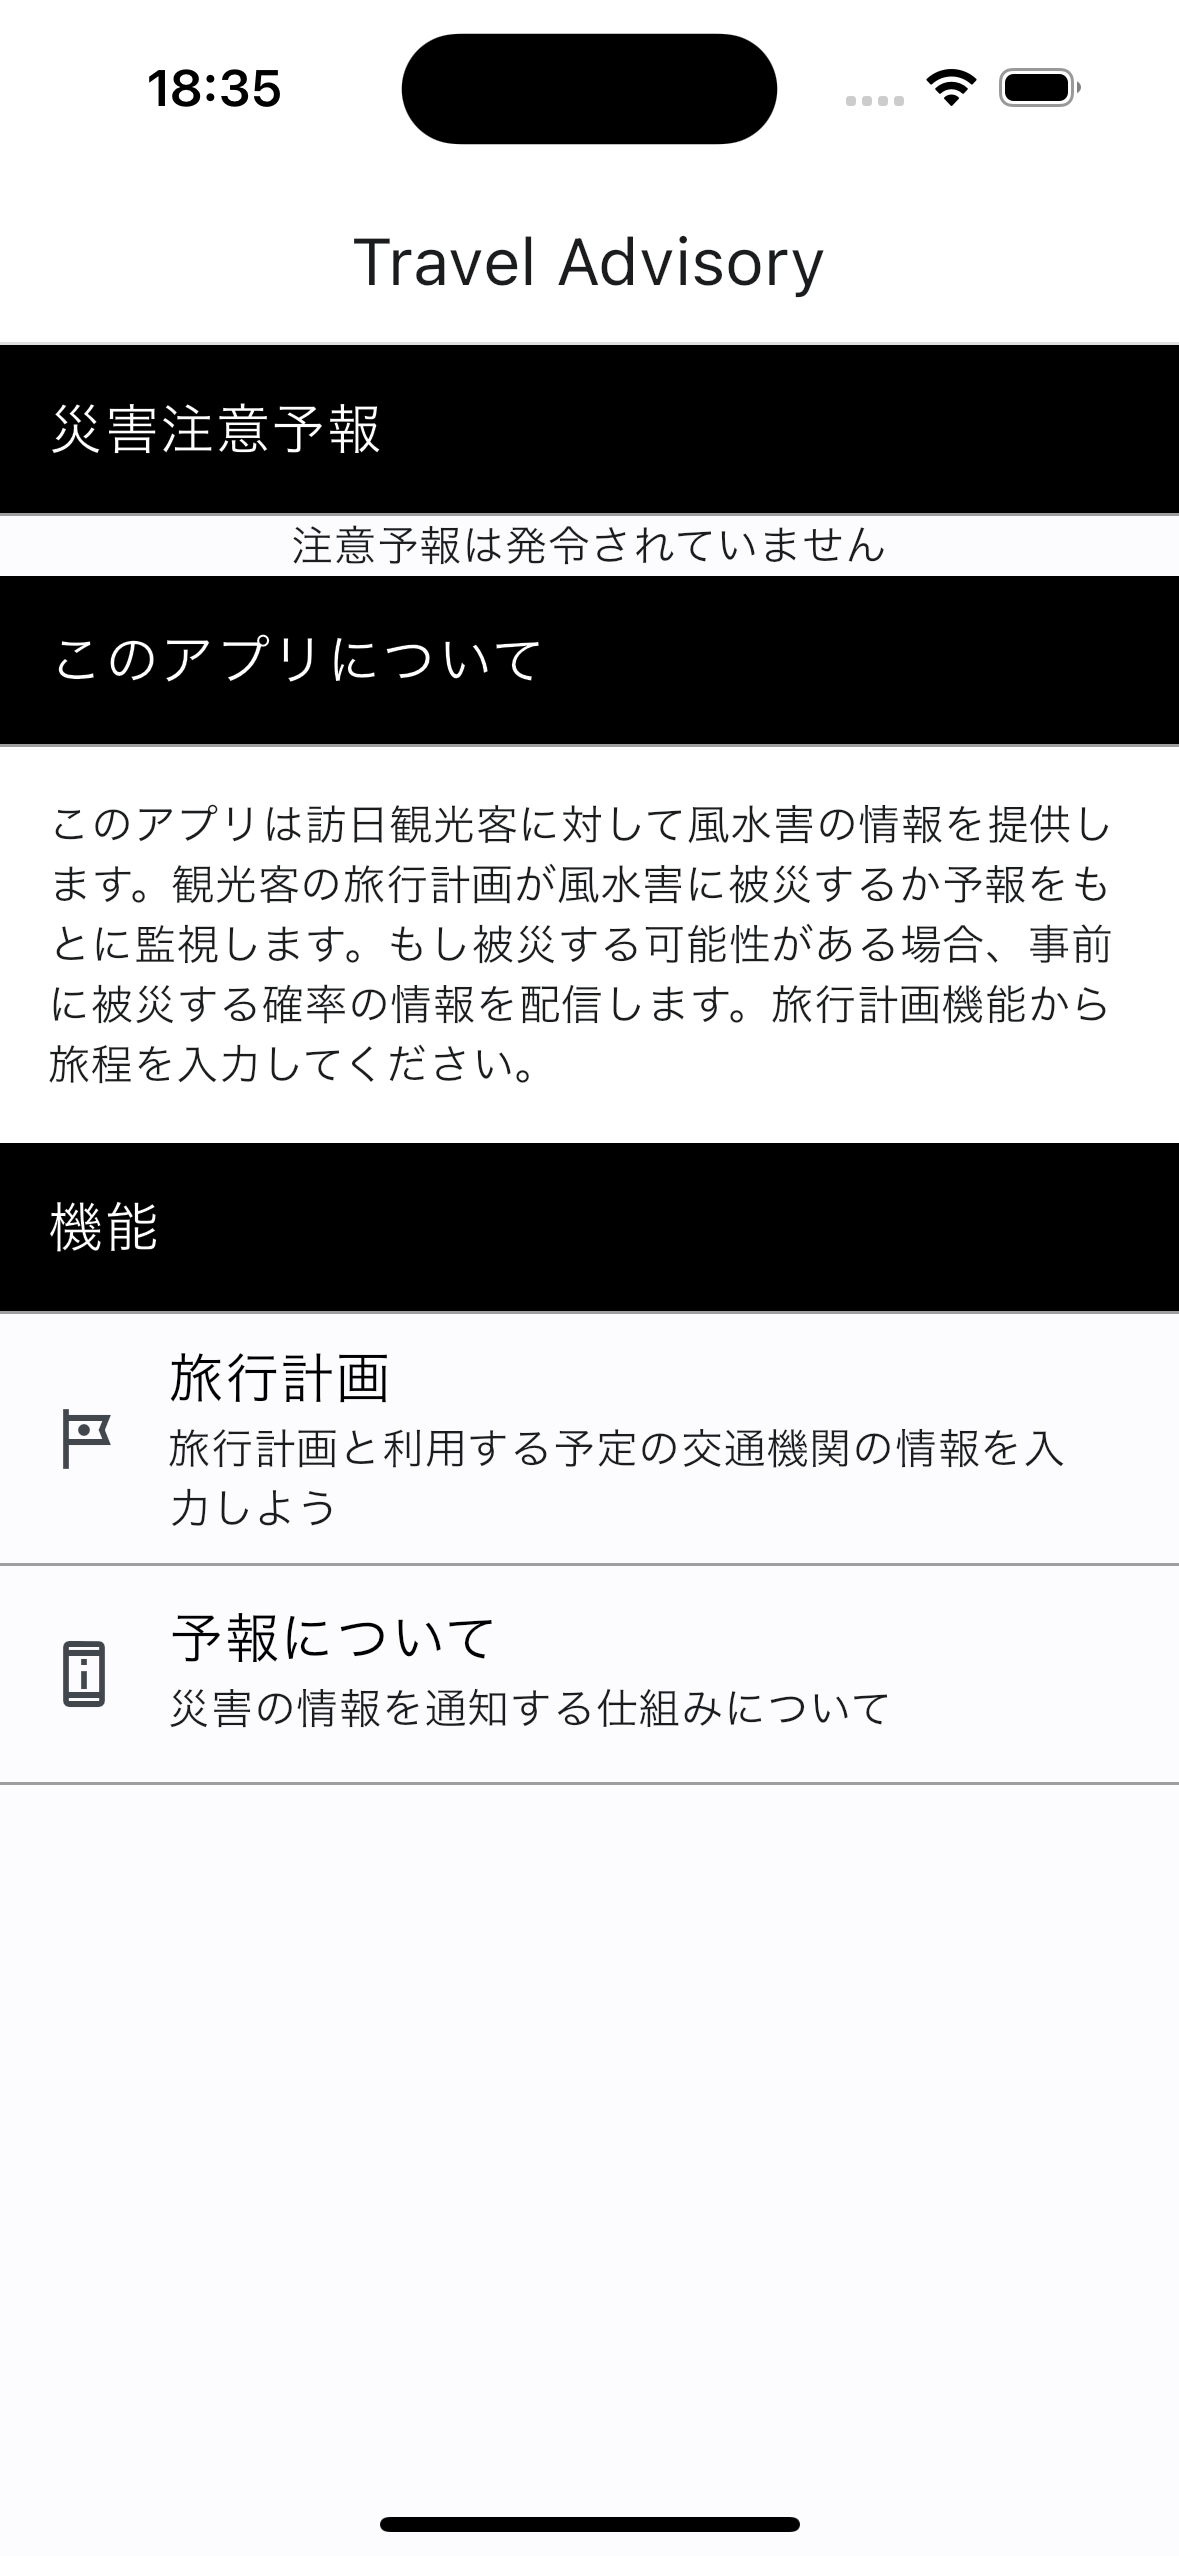
\includegraphics[height=10cm]{./fig/normal_home_screen.png}
  %\vspace{-3mm}
  \caption{通常時のホーム画面}
  \label{fig:normal_home_screen}
  %\vspace{2mm}
\end{figure}

% \subsection{予報についての画面}
% 予報についての画面はアプリケーションが提供する災害注意予報について説明している画面である。
% アプリでの予報の表示の仕方や、気象庁防災情報XMLについて簡単に説明している。

% \begin{figure}[H]
%   \centering
%   \includegraphics[height=8cm]{./fig/forcast_screen_1.png}
%   %\vspace{-3mm}
%   \caption{予報についての画面の図1}
%   \label{fig:forecast_screen_1}
%   %\vspace{2mm}
% \end{figure}

% \begin{figure}[H]
%   \centering
%   \includegraphics[height=8cm]{./fig/forcast_screen_2.png}
%   %\vspace{-3mm}
%   \caption{予報についての画面の図2}
%   \label{fig:forecast_screen_2}
%   %\vspace{2mm}
% \end{figure}

\subsection {旅程パッケージを作成する}
旅程データを作成するために旅程パッケージを作成する.
旅程パッケージ画面は作成した旅程パッケージの一覧と旅行パッケージの作成機能を提供している画面である.
旅行パッケージは右下の計画の作成ボタンをタップすると旅行パッケージ作成画面に遷移して作成できる.
旅行パッケージの一覧からパッケージをタップすると,旅程データ画面に遷移する.

\begin{figure}[H]
  \begin{minipage}[b]{0.45\linewidth}
    \centering
    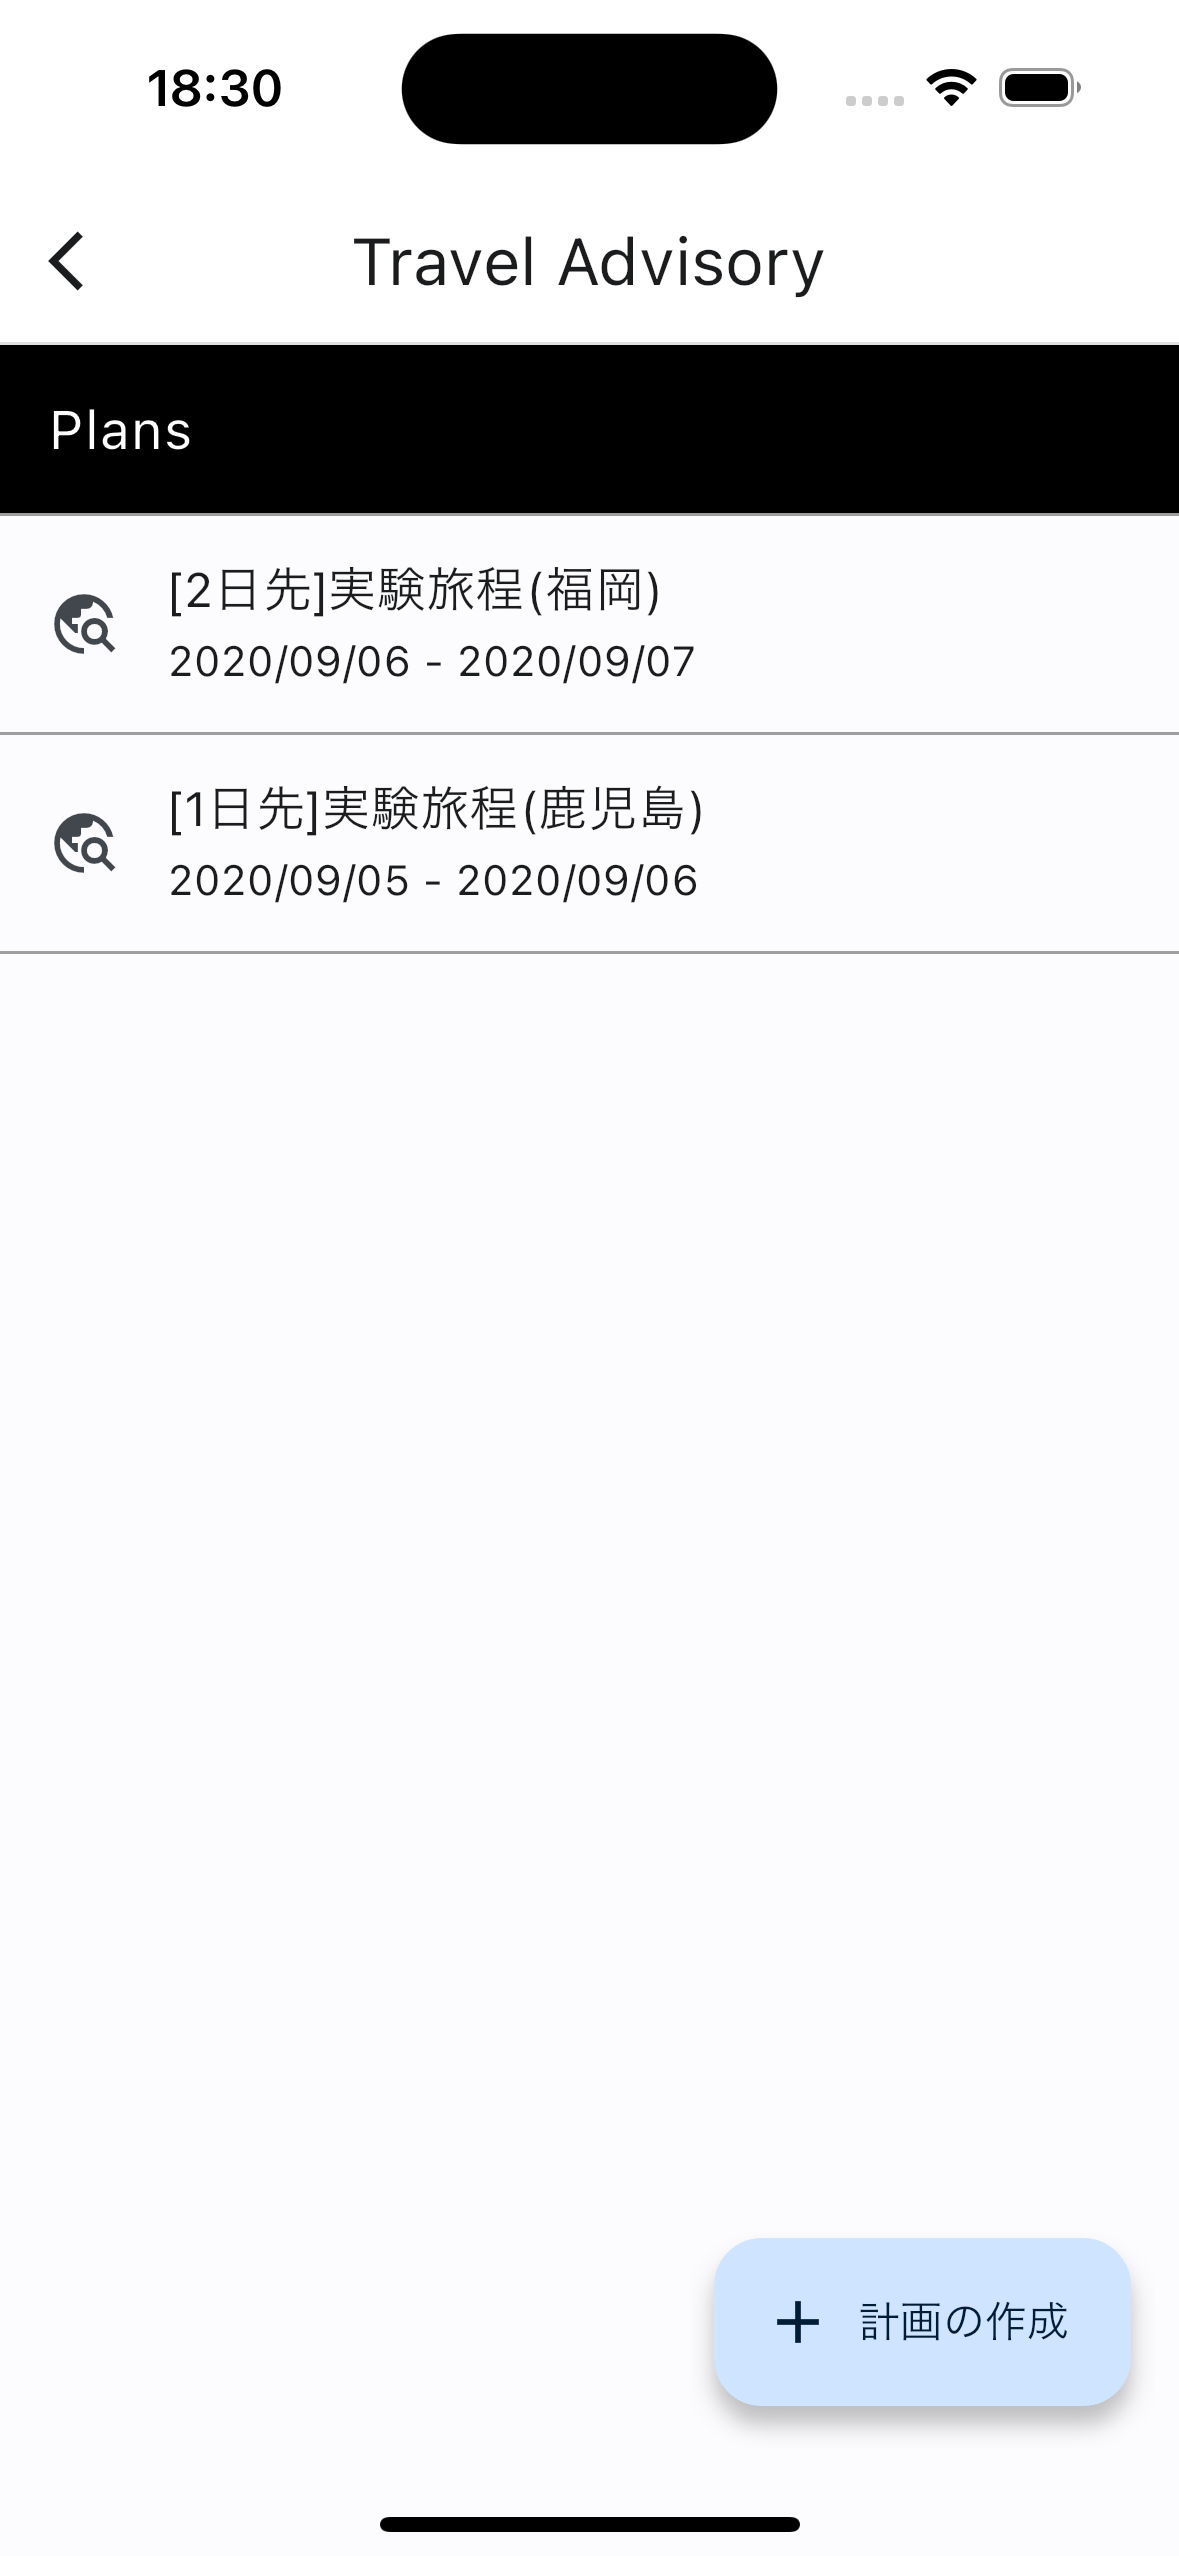
\includegraphics[height=10cm]{./fig/travel_pack_list.png}
    %\vspace{-3mm}
    \caption{旅程パッケージ画面}
    \label{fig:travel_pack_list}
    %\vspace{2mm}
  \end{minipage}
  \begin{minipage}[b]{0.45\linewidth}
    \centering
    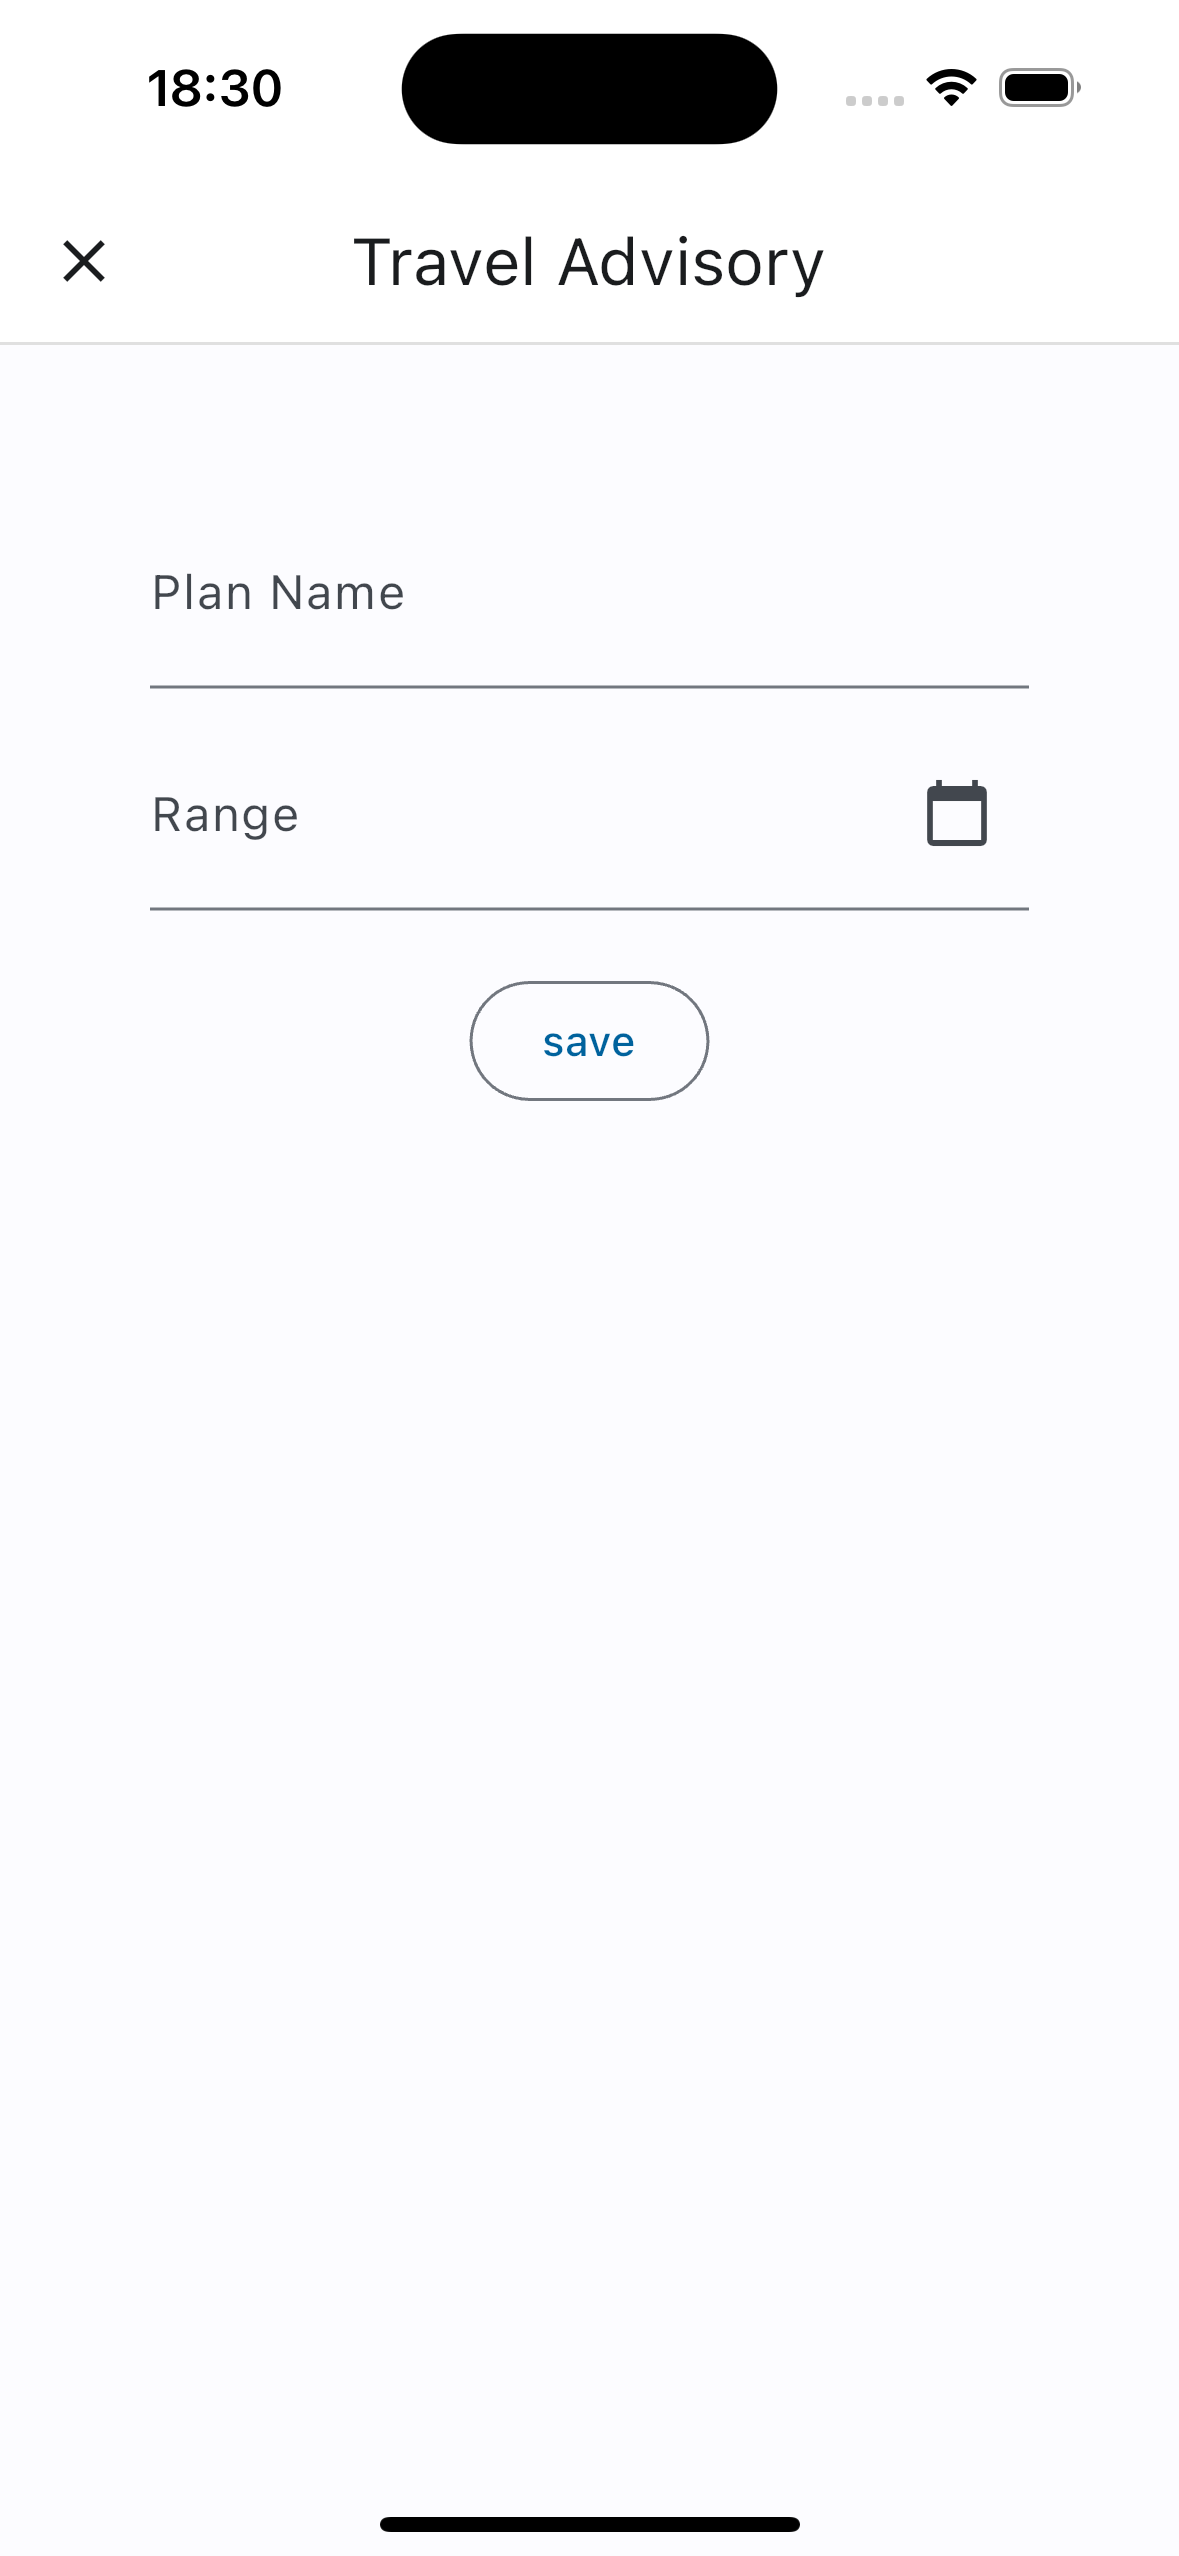
\includegraphics[height=10cm]{./fig/travel_pack_create.png}
    %\vspace{-3mm}
    \caption{旅程パッケージ作成画面}
    \label{fig:travel_pack_create}
    %\vspace{2mm}
  \end{minipage}
\end{figure}

\subsection {旅程データを作成する}
旅程パッケージに旅程データを作成し,登録する.
旅程データ画面は日付ごとに作成した旅程データの一覧と場所・交通データの作成機能を提供している画面である.
下部のAdd Spotボタンをタップすると場所データの作成が,Add Transportationボタンをタップすると交通データの作成画面に遷移する.

\begin{figure}[H]
  \centering
  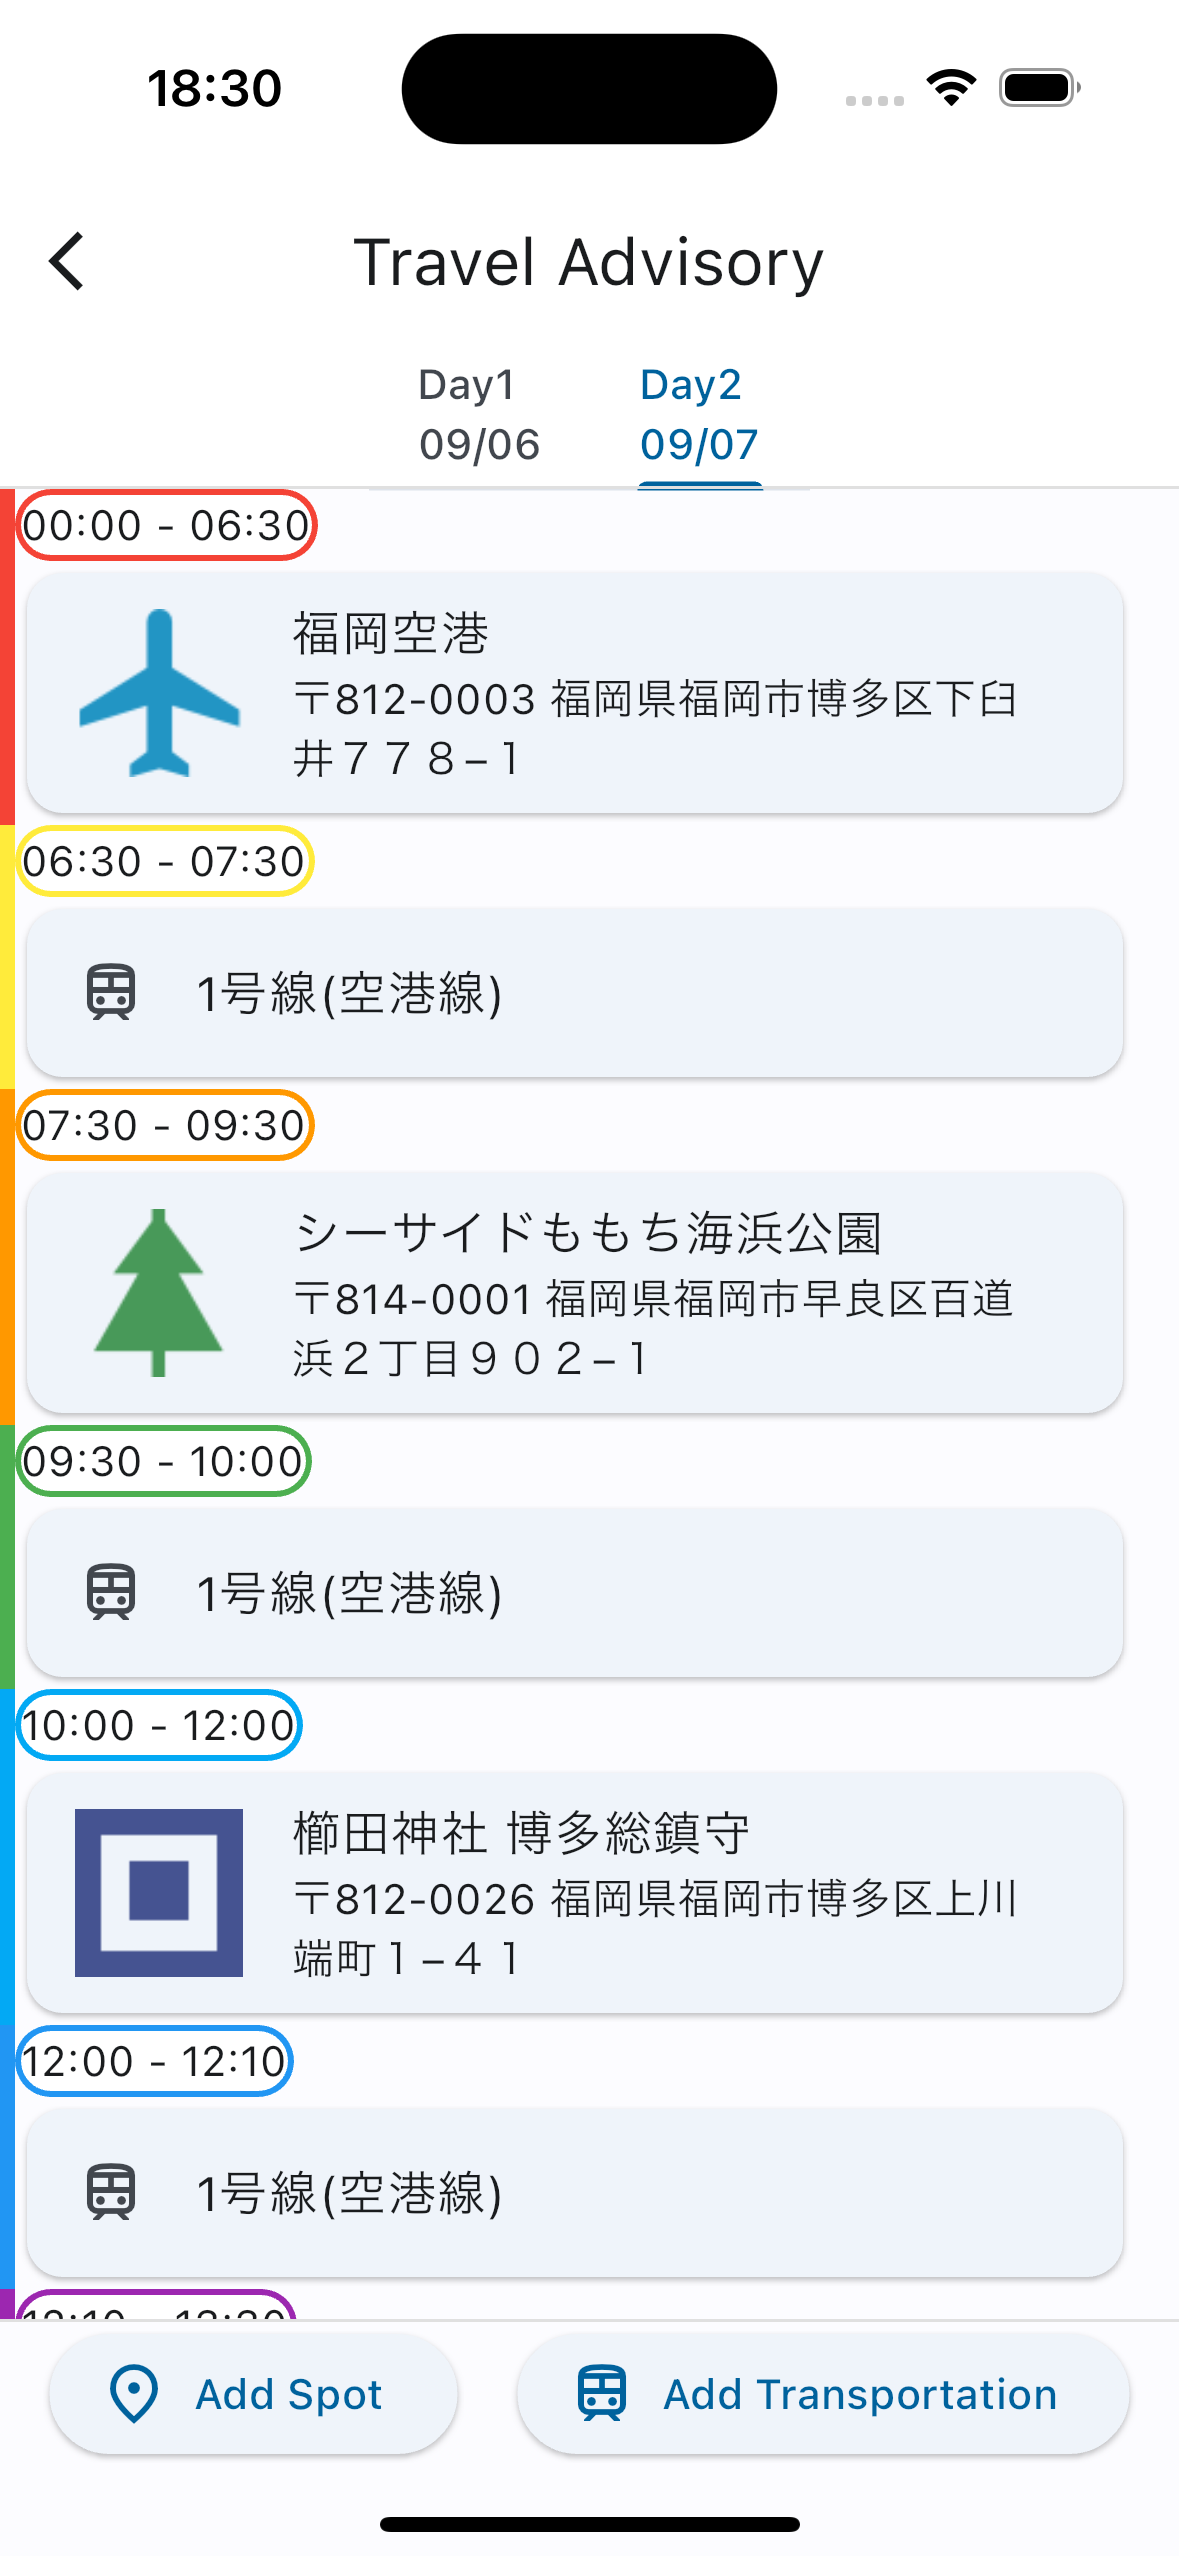
\includegraphics[height=10cm]{./fig/travel_data_list.png}
  %\vspace{-3mm}
  \caption{旅程データ画面}
  \label{fig:travel_data_list}
  %\vspace{2mm}
\end{figure}

\subsubsection {場所データの作成}
場所データを作成する.
訪れる予定の場所を検索する機能とその時刻を入力する機能を提供している画面である.
検索機能はGoogle Map Apiを利用している.
検索すると場所の候補が複数表示されるので,1つを選択してSaveボタンを押す.

\begin{figure}[H]
  \centering
  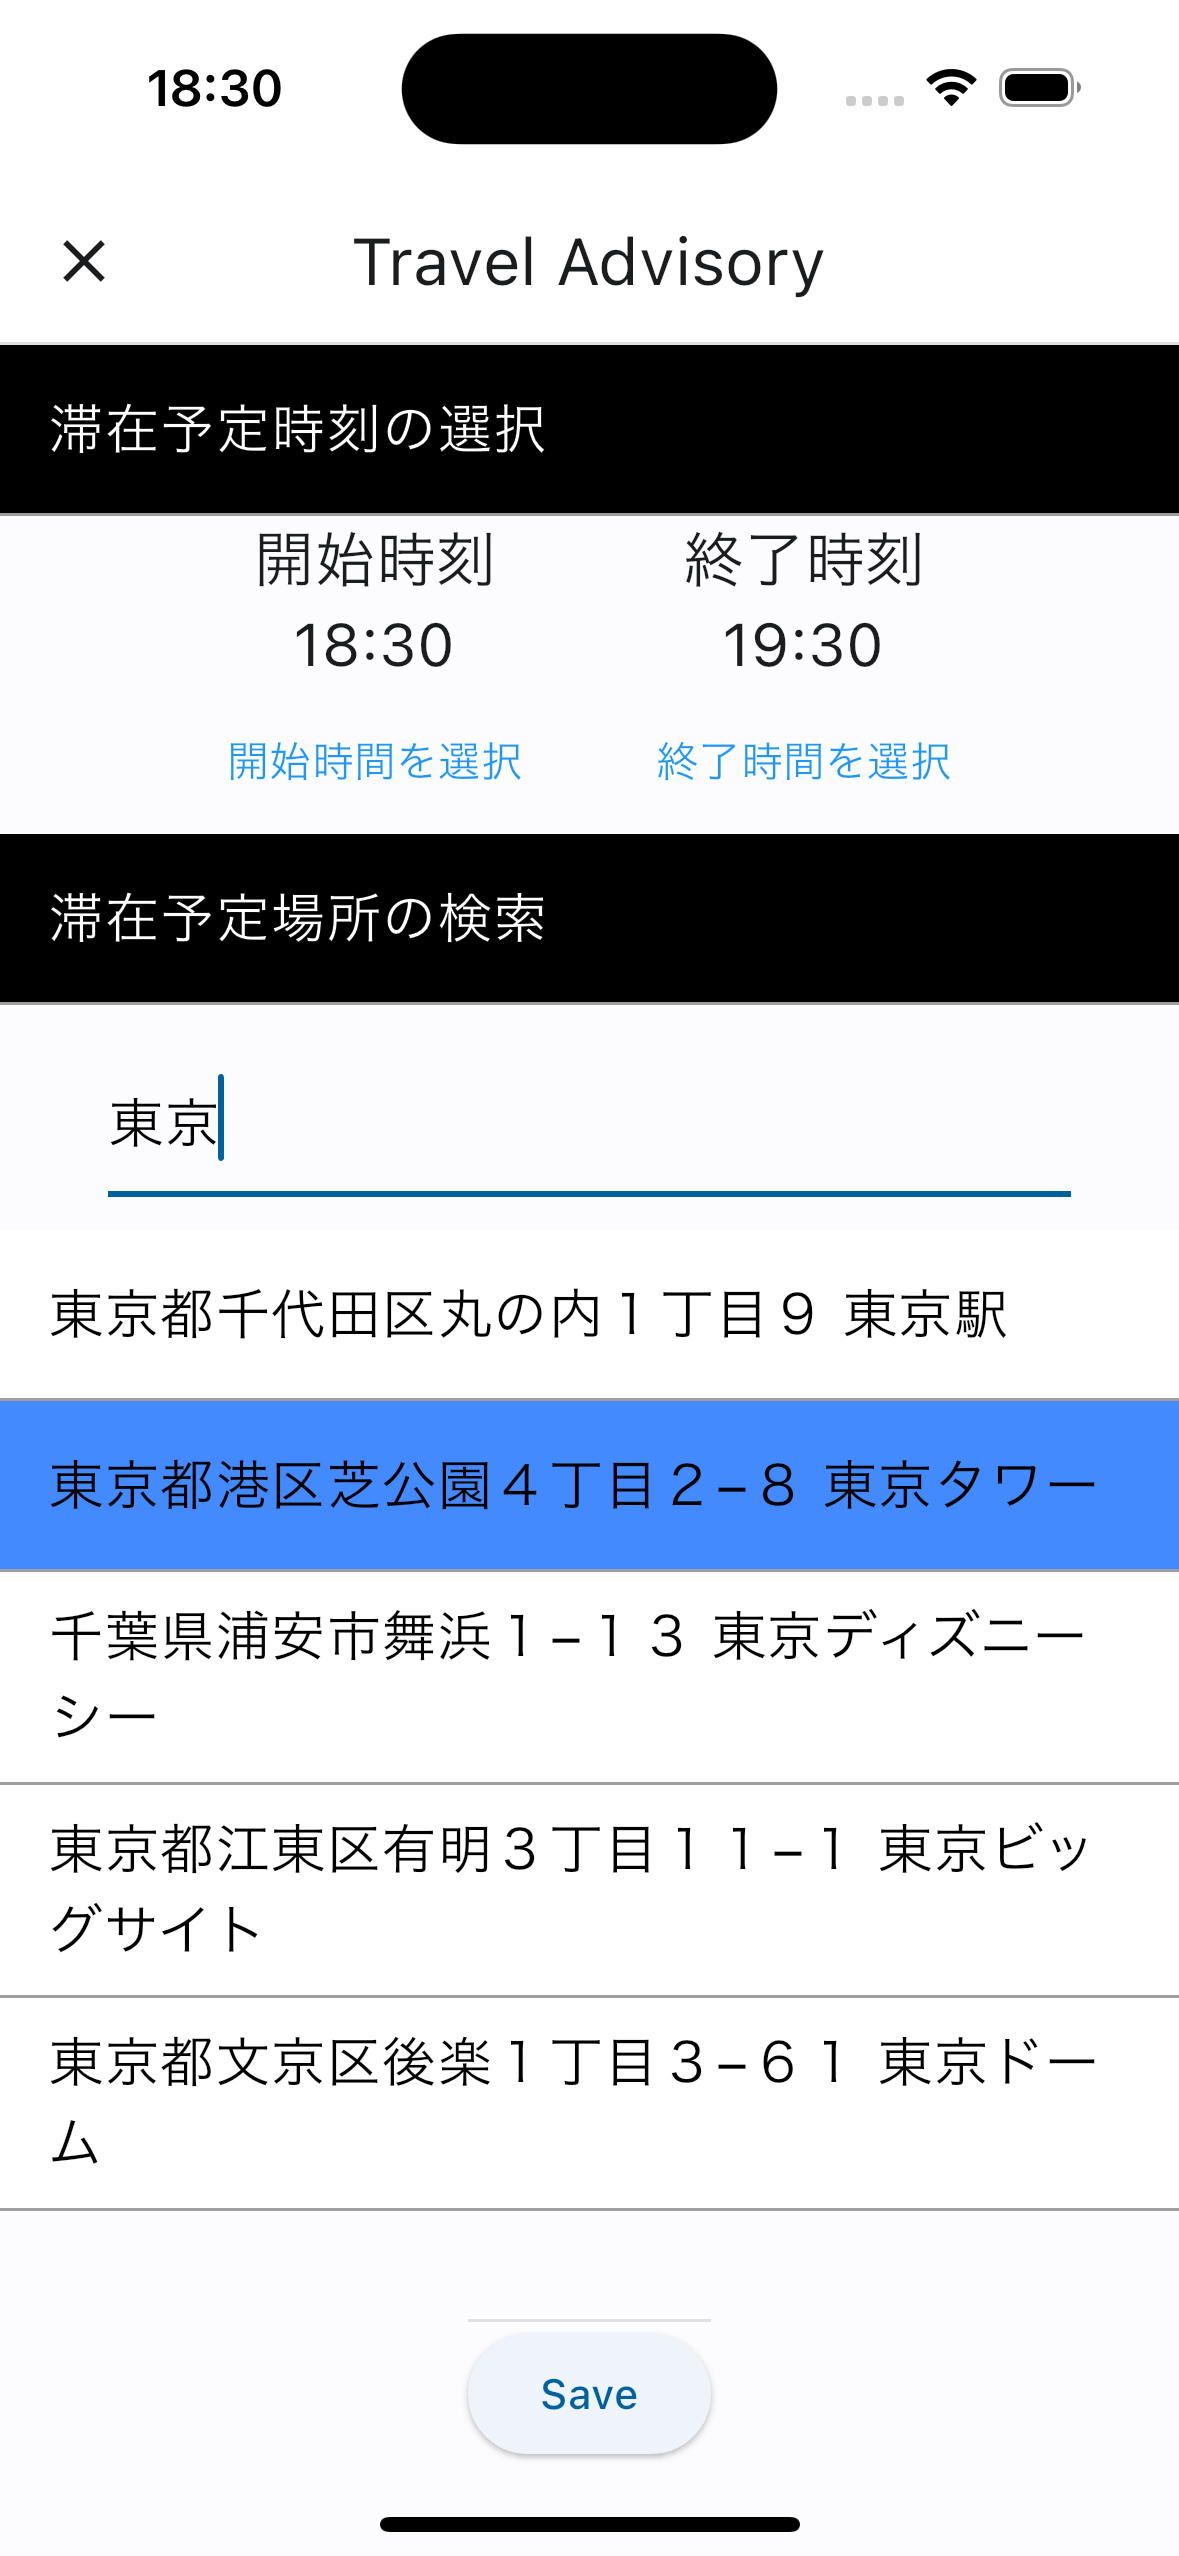
\includegraphics[height=10cm]{./fig/spot_data_save.png}
  %\vspace{-3mm}
  \caption{場所データの作成画面}
  \label{fig:spot_data_save}
  %\vspace{2mm}
\end{figure}

\subsubsection {交通機関データの作成}
交通データを作成する.
利用する予定の鉄道の路線を検索する機能を提供する.
路線を選択した後,路線に属する駅の一覧が表示される.
自分が利用する予定の駅を1つ以上選択し,時刻とともにデータを保存する.

\begin{figure}[H]
  \begin{minipage}[b]{0.45\linewidth}
    \centering
    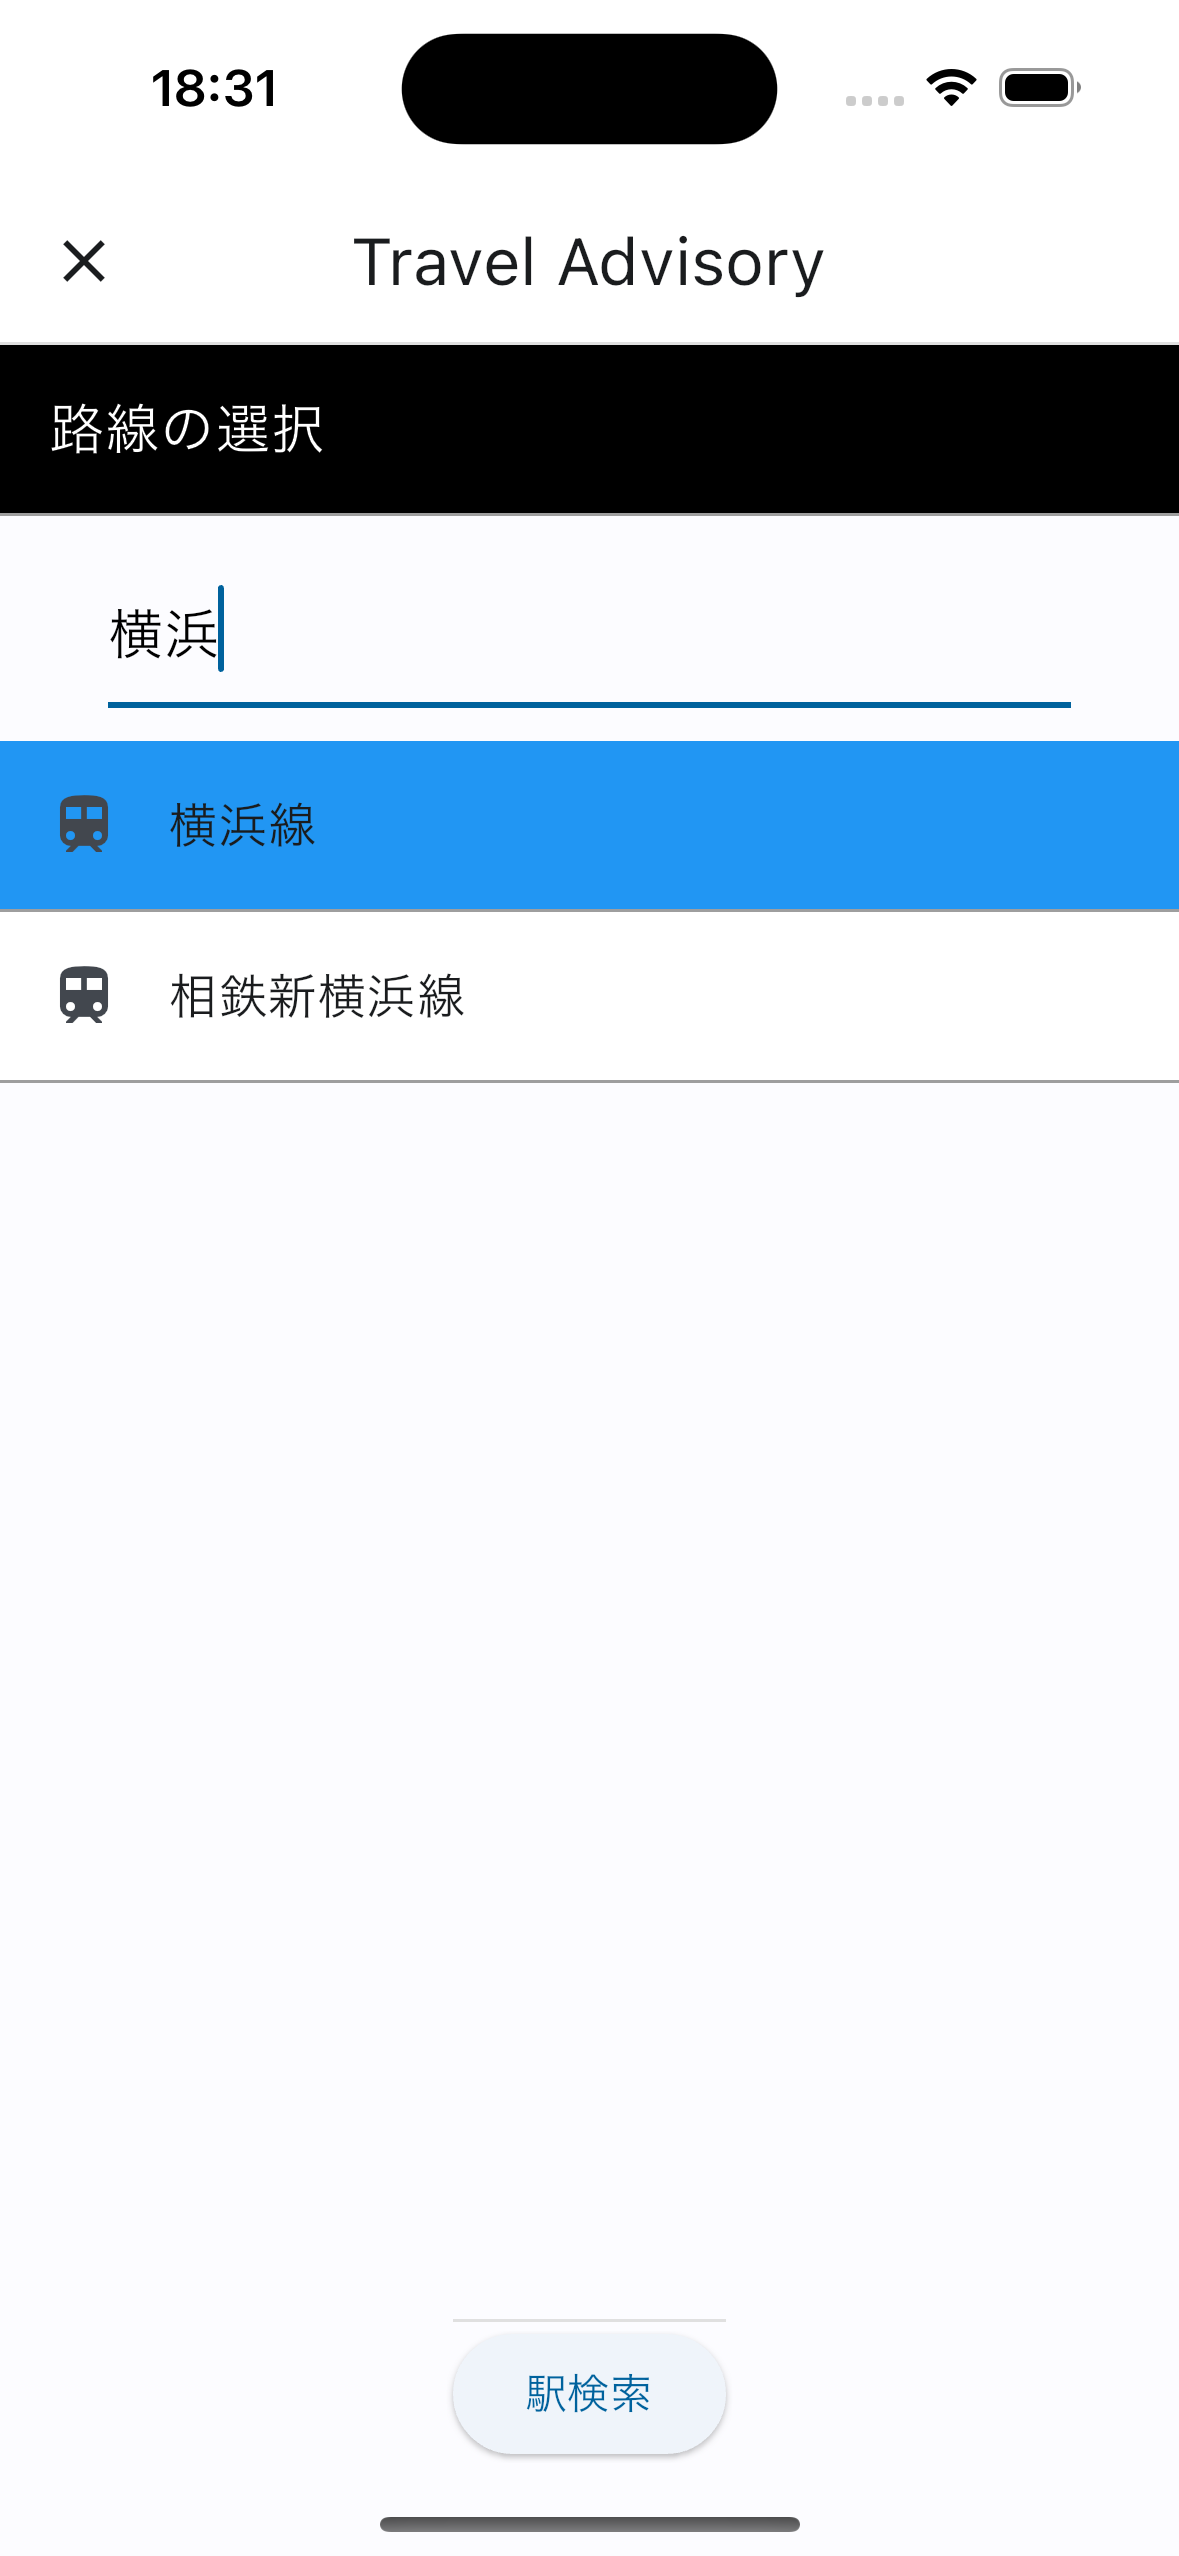
\includegraphics[height=10cm]{./fig/railway_search.png}
    %\vspace{-3mm}
    \caption{鉄道の路線を検索する画面}
    \label{fig:railway_search}
    %\vspace{2mm}
  \end{minipage}
  \begin{minipage}[b]{0.45\linewidth}
    \centering
    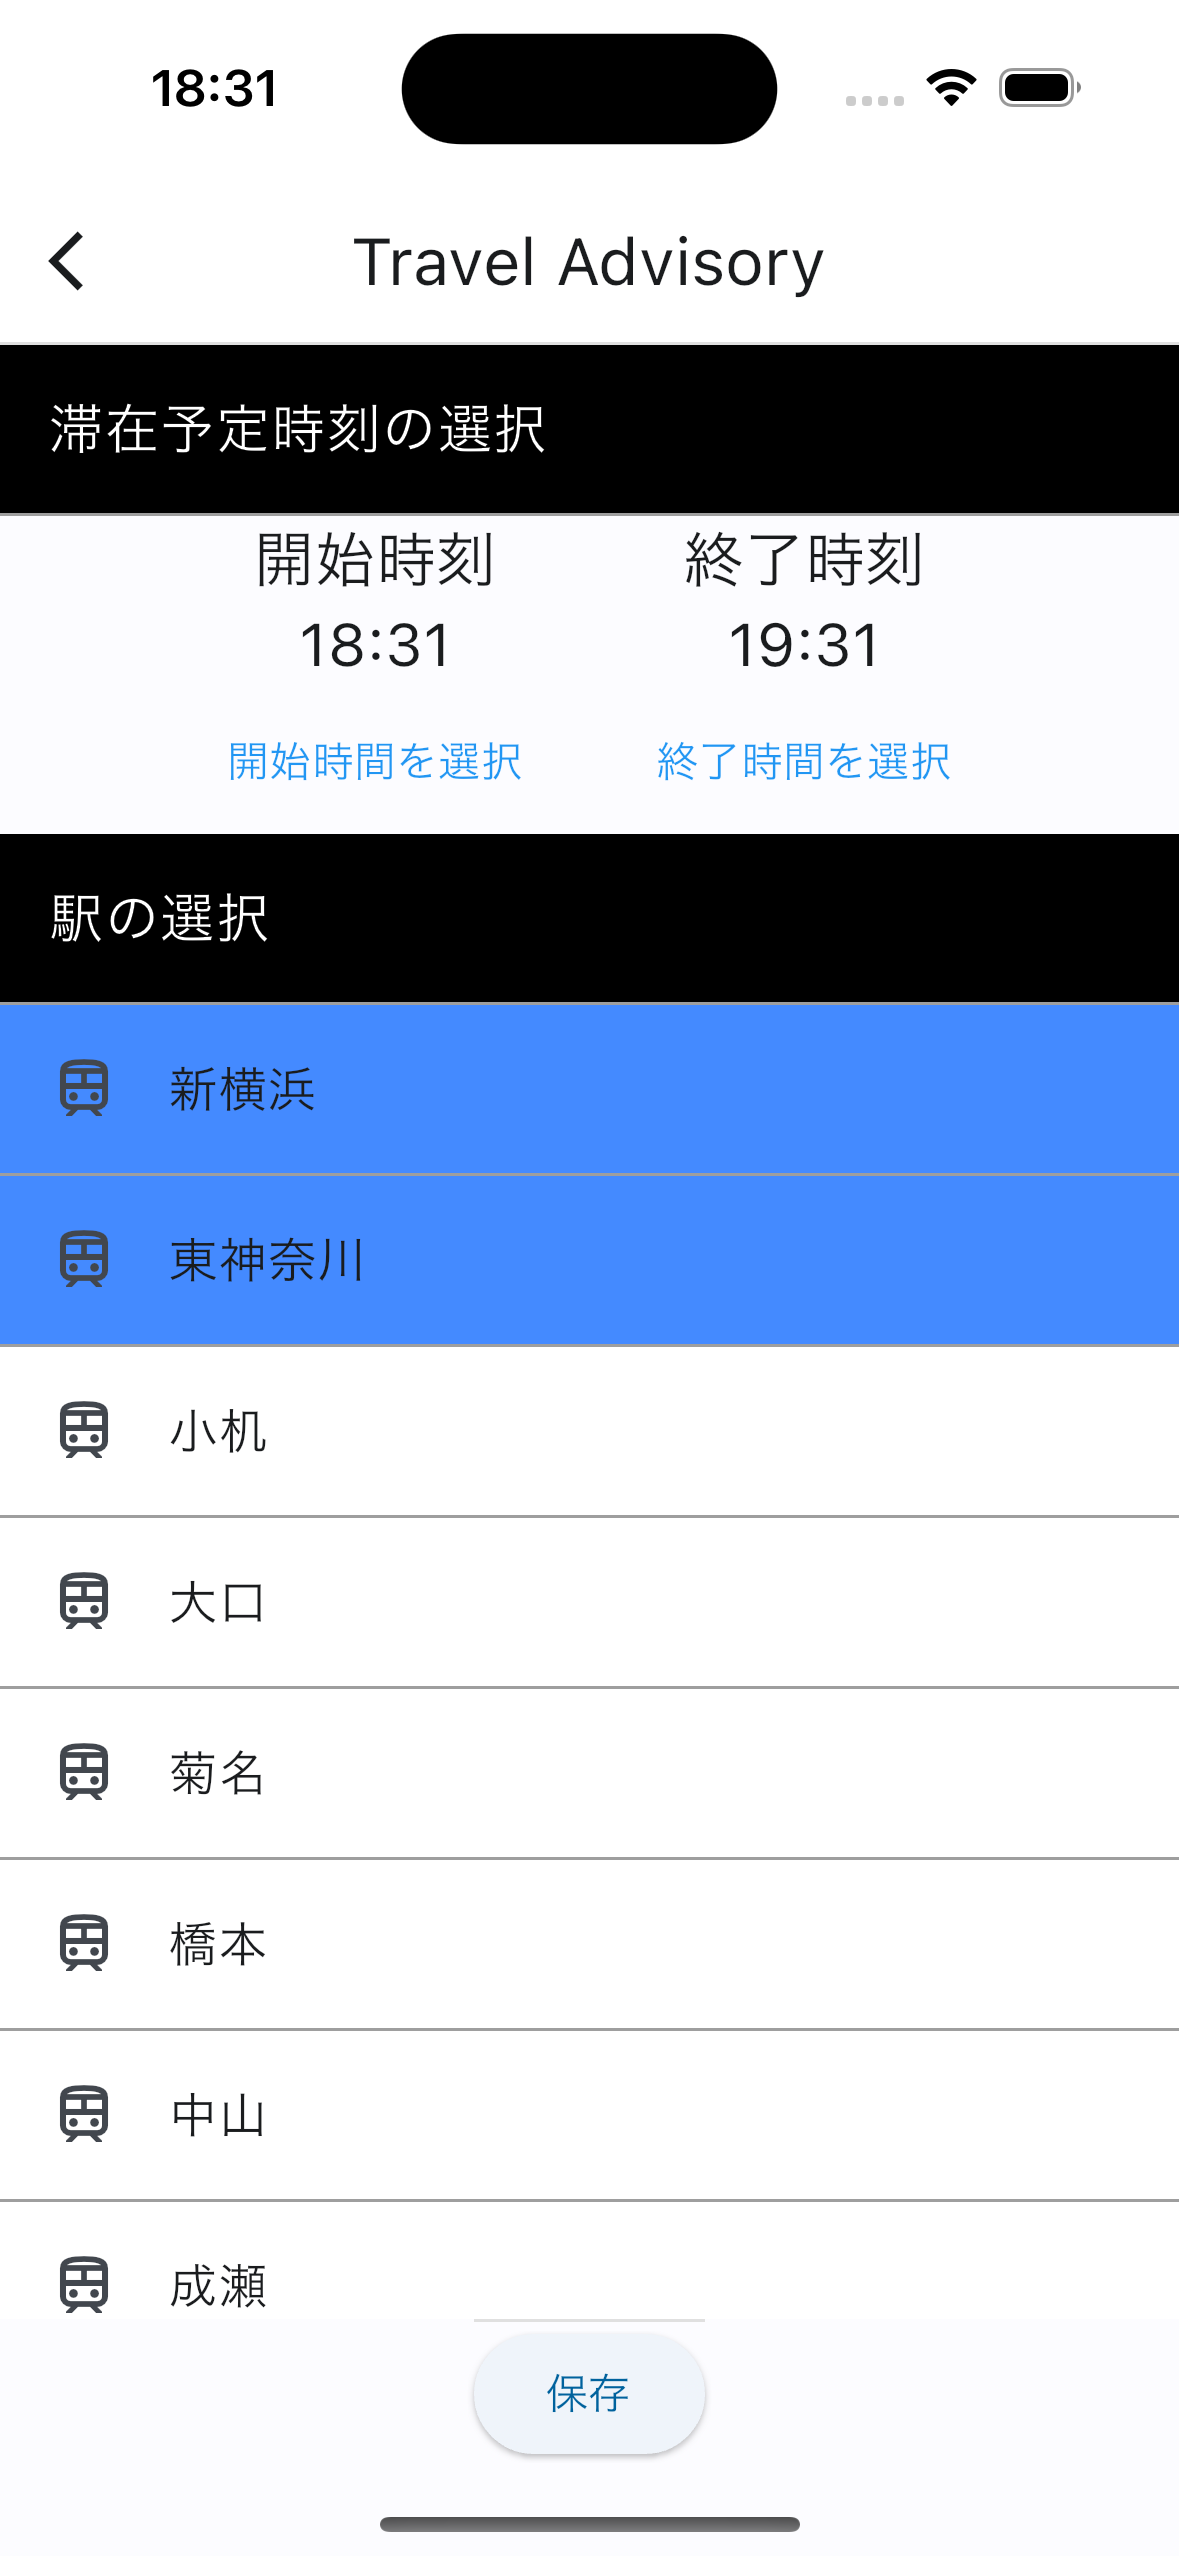
\includegraphics[height=10cm]{./fig/trans_data_save.png}
    %\vspace{-3mm}
    \caption{利用する駅を保存する画面}
    \label{fig:trans_data_save}
    %\vspace{2mm}
  \end{minipage}
\end{figure}

\subsection {通知を受け取る}
通知をタップする.
保存した旅程データがバッチ処理によって災害情報と紐付けられると,push通知が届く.
そしてホーム画面の災害注意予報一覧から注意報が出ている旅程パッケージをタップする.
なお,本アプリにおいては遠隔からの通知を受け取る仕様ではなく,ユーザがアプリを通じて通知を送信する.
本来であれば遠隔から通知を受け取るべきだが,後述する評価実験に関係のない機能であることから本実験では実装を見送った.

\begin{figure}[H]
  \begin{minipage}[b]{0.45\linewidth}
    \centering
    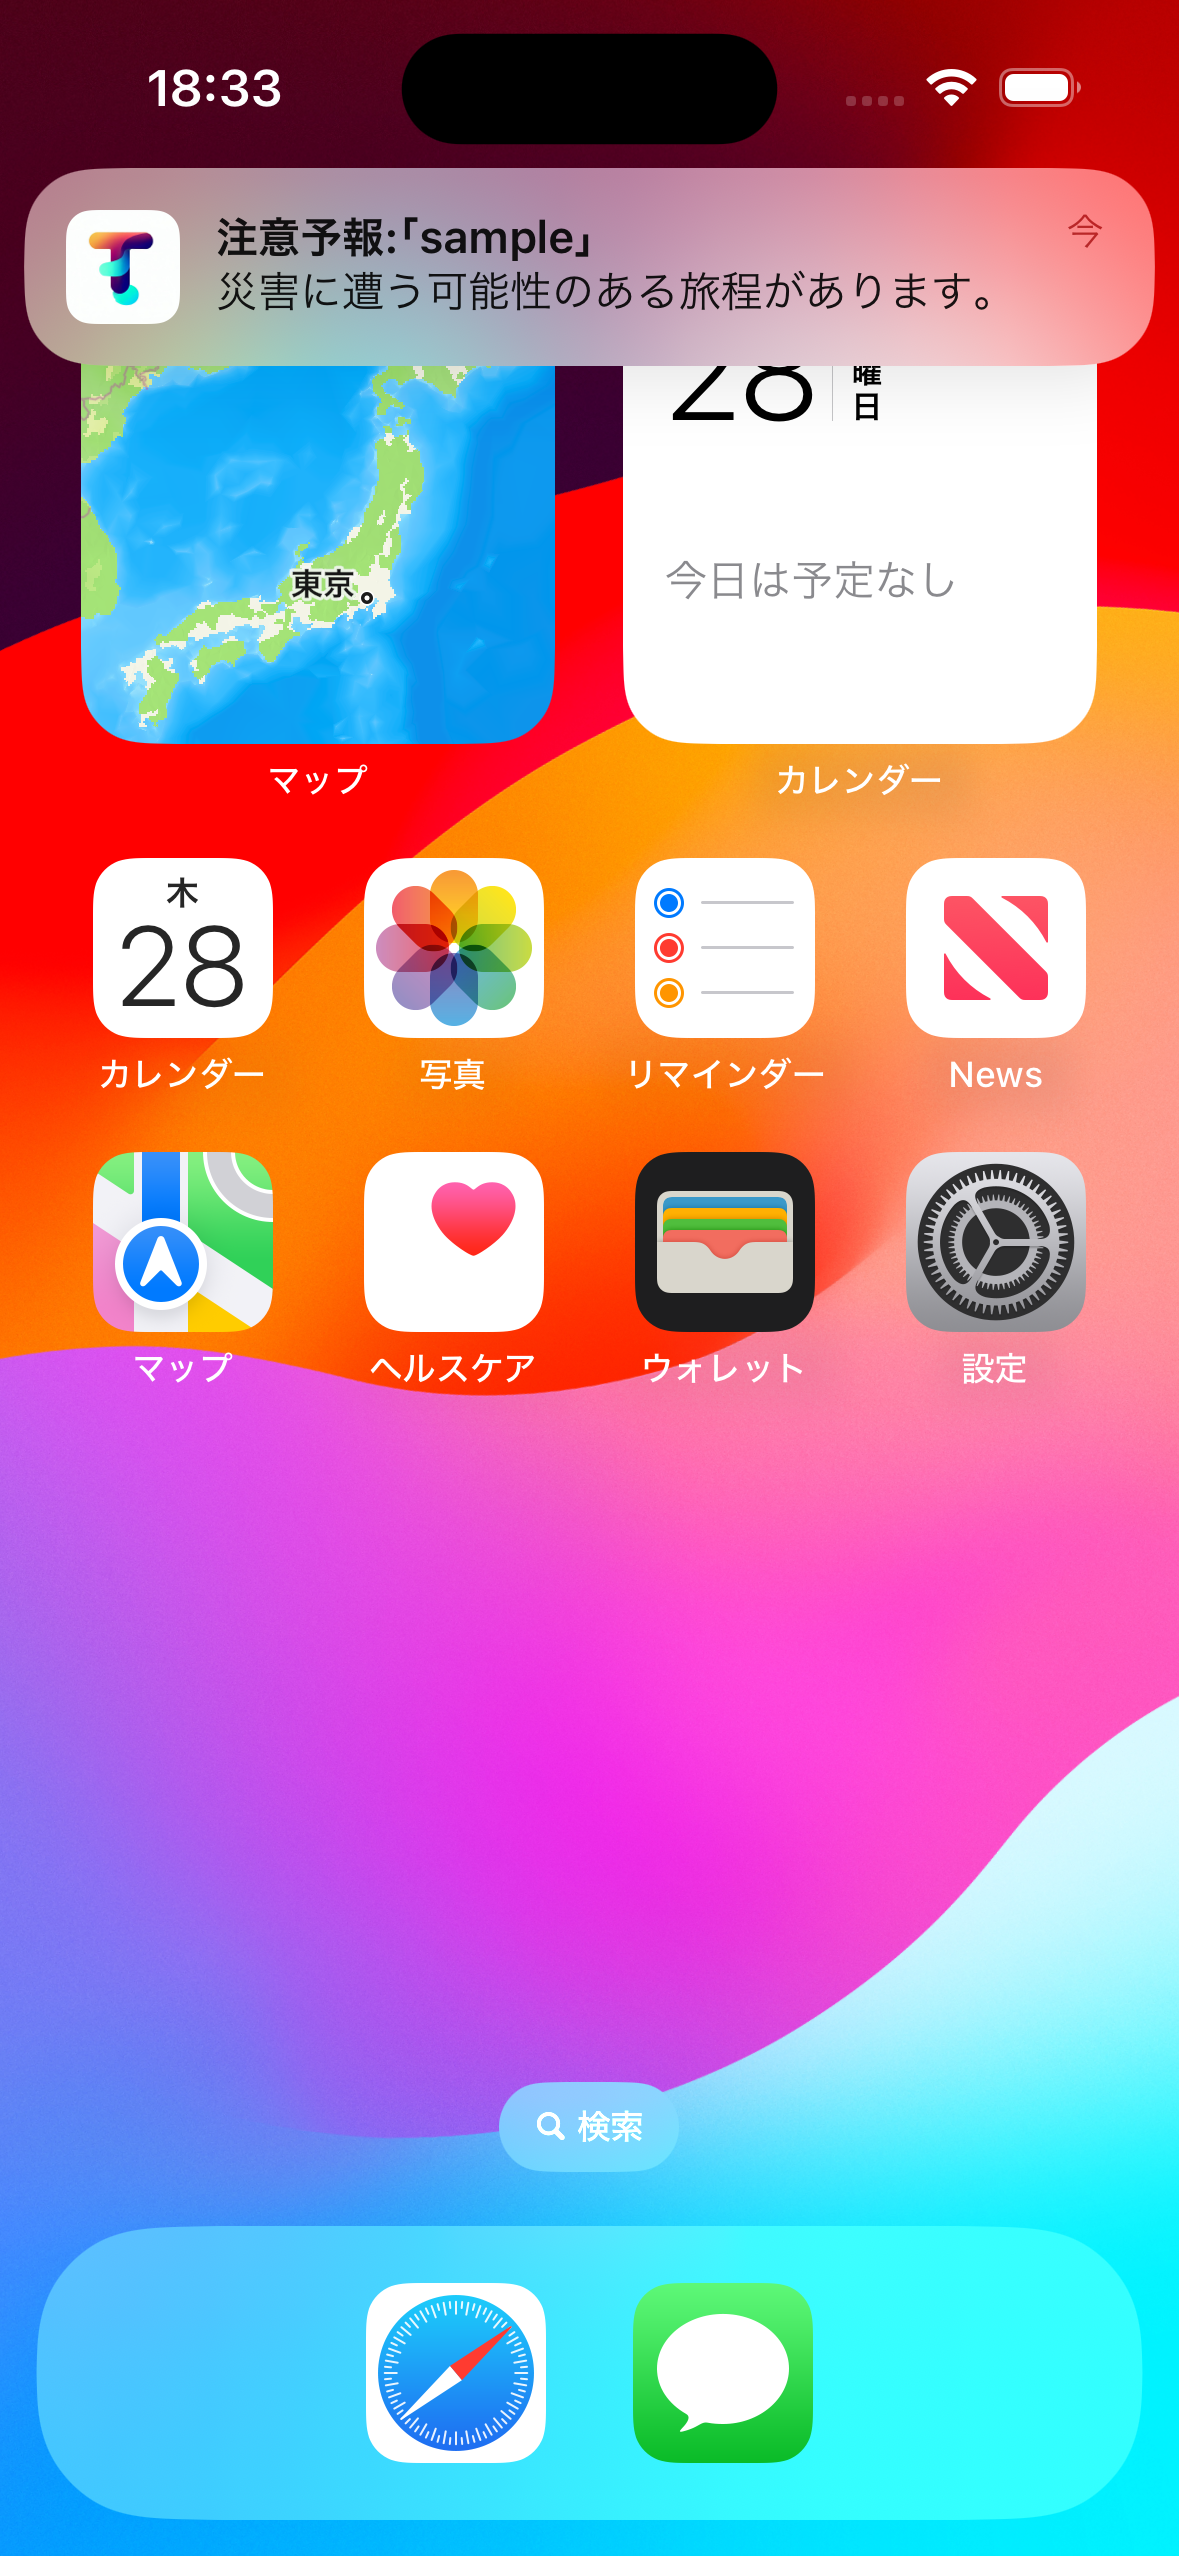
\includegraphics[height=10cm]{./fig/notion.png}
    %\vspace{-3mm}
    \caption{通知の表示}
    \label{fig:notion}
    %\vspace{2mm}
  \end{minipage}
  \begin{minipage}[b]{0.45\linewidth}
    \centering
    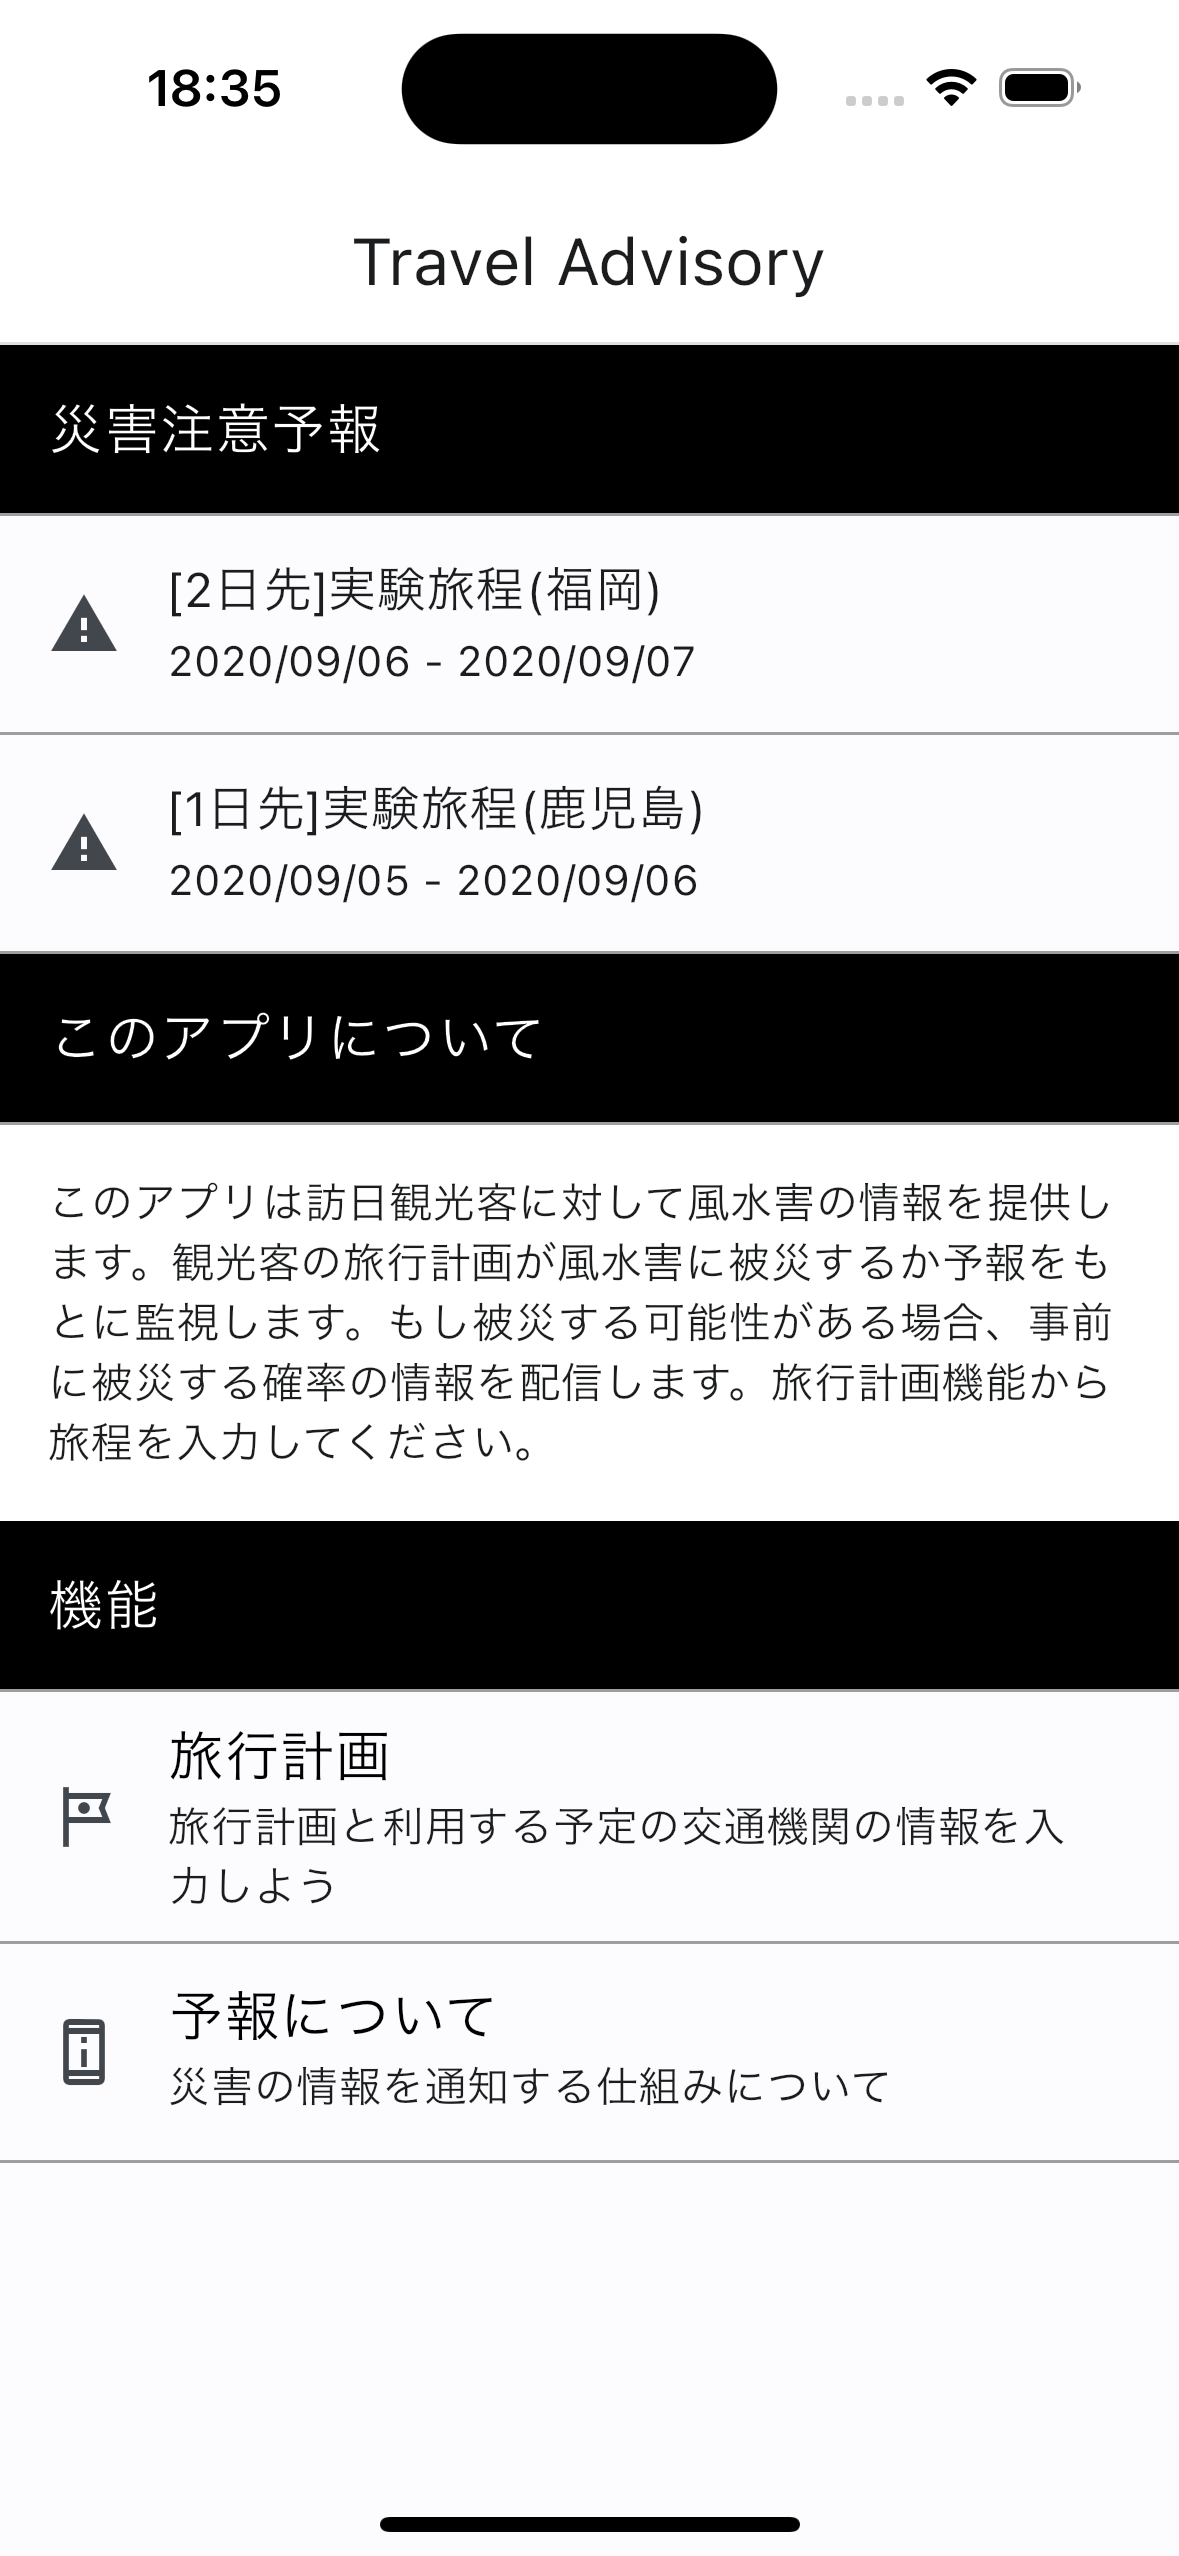
\includegraphics[height=10cm]{./fig/unormal_home_screen.png}
    %\vspace{-3mm}
    \caption{災害注意予報通知時のホーム画面}
    \label{fig:unormal_home_screen}
    %\vspace{2mm}
  \end{minipage}
\end{figure}

\subsection {災害注意予報を確認する}
選択した旅行パッケージの災害注意予報が紐付けられている旅程データの一覧を閲覧する.
一覧から旅程データを選択する.
\begin{figure}[H]
  \centering
  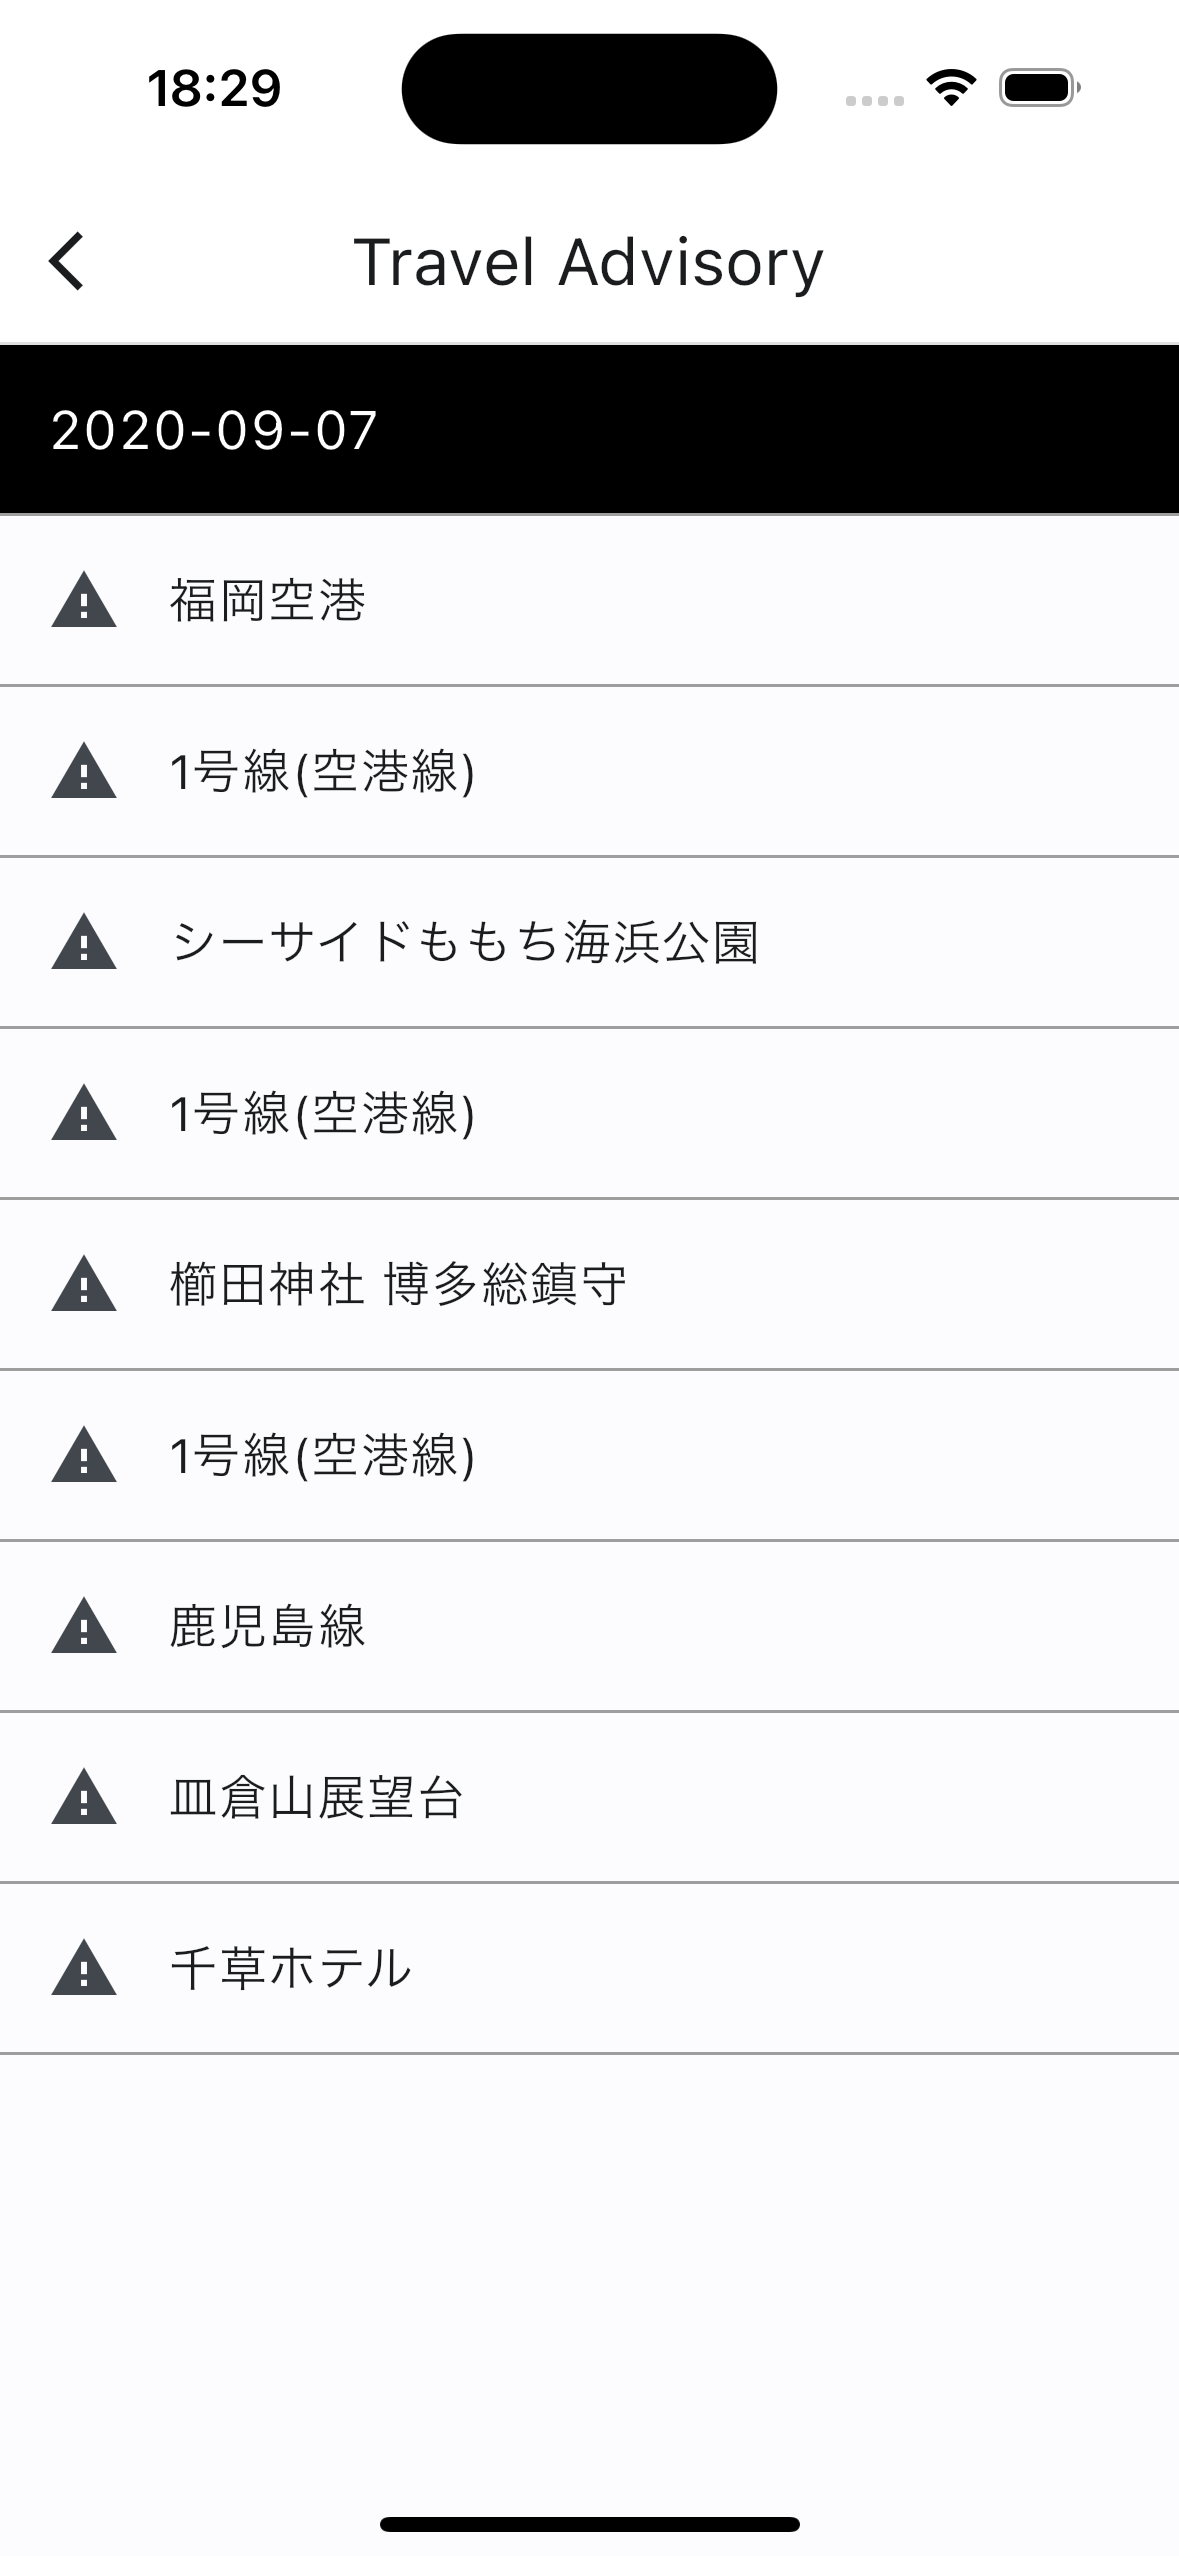
\includegraphics[height=10cm]{./fig/advisory_data_list.png}
  %\vspace{-3mm}
  \caption{災害注意予報が出ている旅程データの一覧}
  \label{fig:advisory_data_list}
  %\vspace{2mm}
\end{figure}

\subsubsection {場所データの災害注意予報}
場所データに対する災害注意予報を閲覧する.
提供される災害の種類は雨と風(風雪)である.災害の種類ごとに災害が起こる確率を提供している.
それぞれの災害のリストをタップすると,ストック情報の画面に遷移する.

\begin{figure}[H]
  \centering
  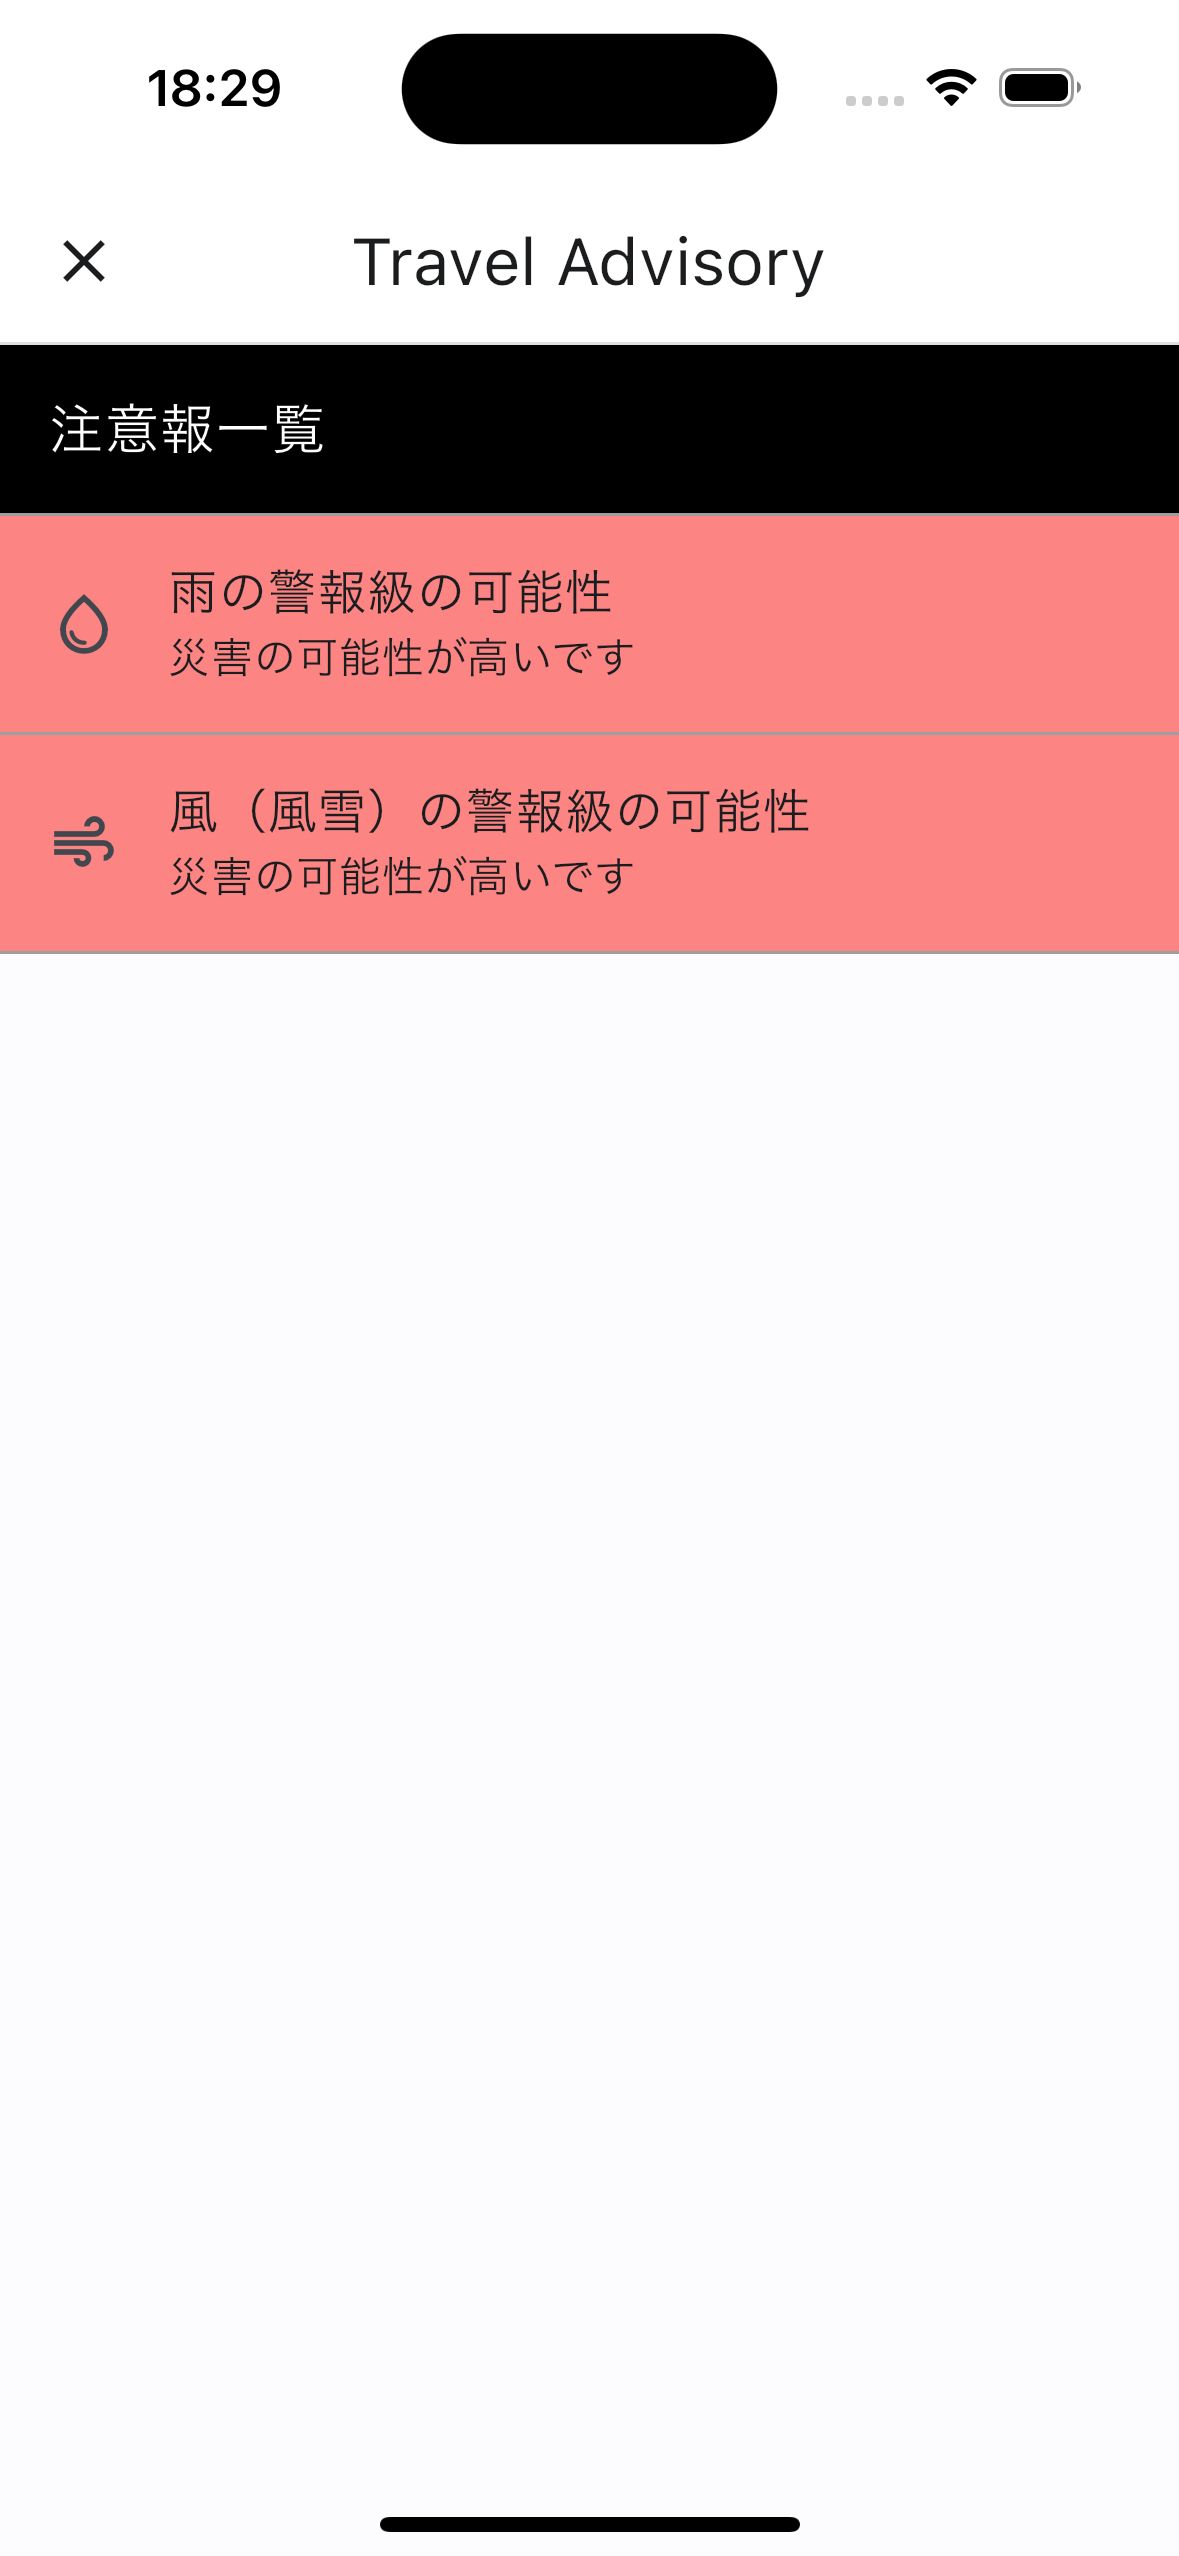
\includegraphics[height=10cm]{./fig/spot_advisory.png}
  %\vspace{-3mm}
  \caption{場所データの災害注意予報画面}
  \label{fig:spot_advisory}
  %\vspace{2mm}
\end{figure}

\subsubsection {交通データの災害注意予報}
交通データに対する災害注意予報を閲覧する.
交通データにおいては,場所データと同じように駅データごとに災害注意予報が提供される.
各駅に対して災害の発生する可能性を運休する可能性として情報を提供している.
さらに,ページ下部には災害時に起こる交通機関の運休の現象や計画運休の現象についての説明がある.

\begin{figure}[H]
  \begin{minipage}[b]{0.45\linewidth}
    \centering
    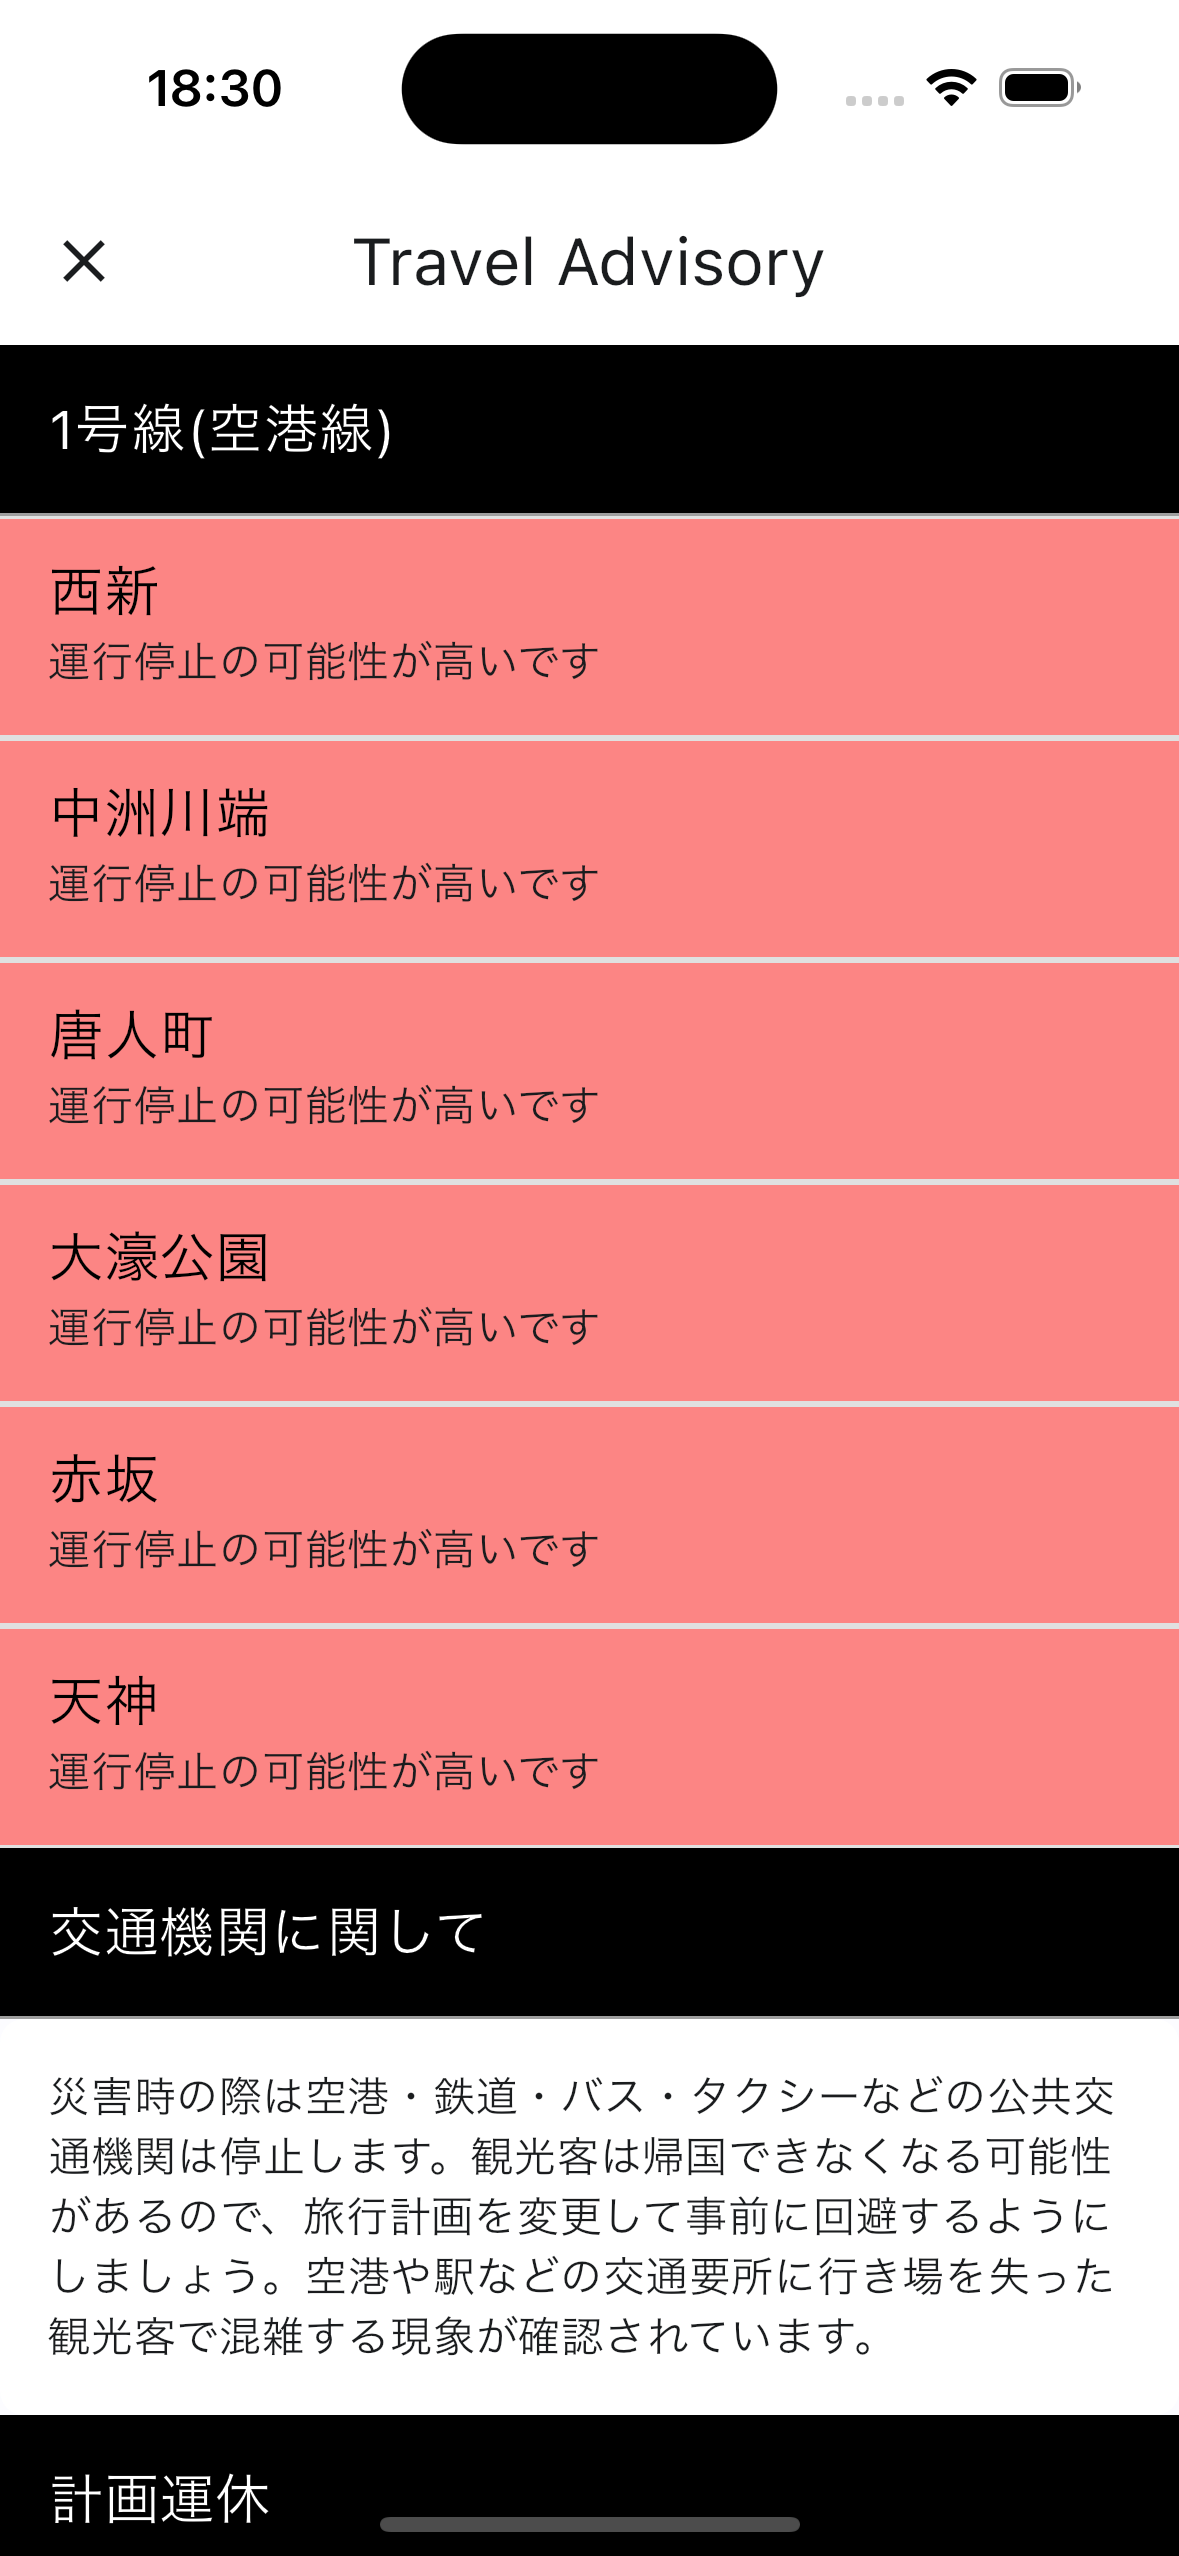
\includegraphics[height=10cm]{./fig/trans_advisory_1.png}
    %\vspace{-3mm}
    \caption{交通データの災害注意予報画面1}
    \label{fig:trans_advisory_1}
    %\vspace{2mm}
  \end{minipage}
  \begin{minipage}[b]{0.45\linewidth}
    \centering
    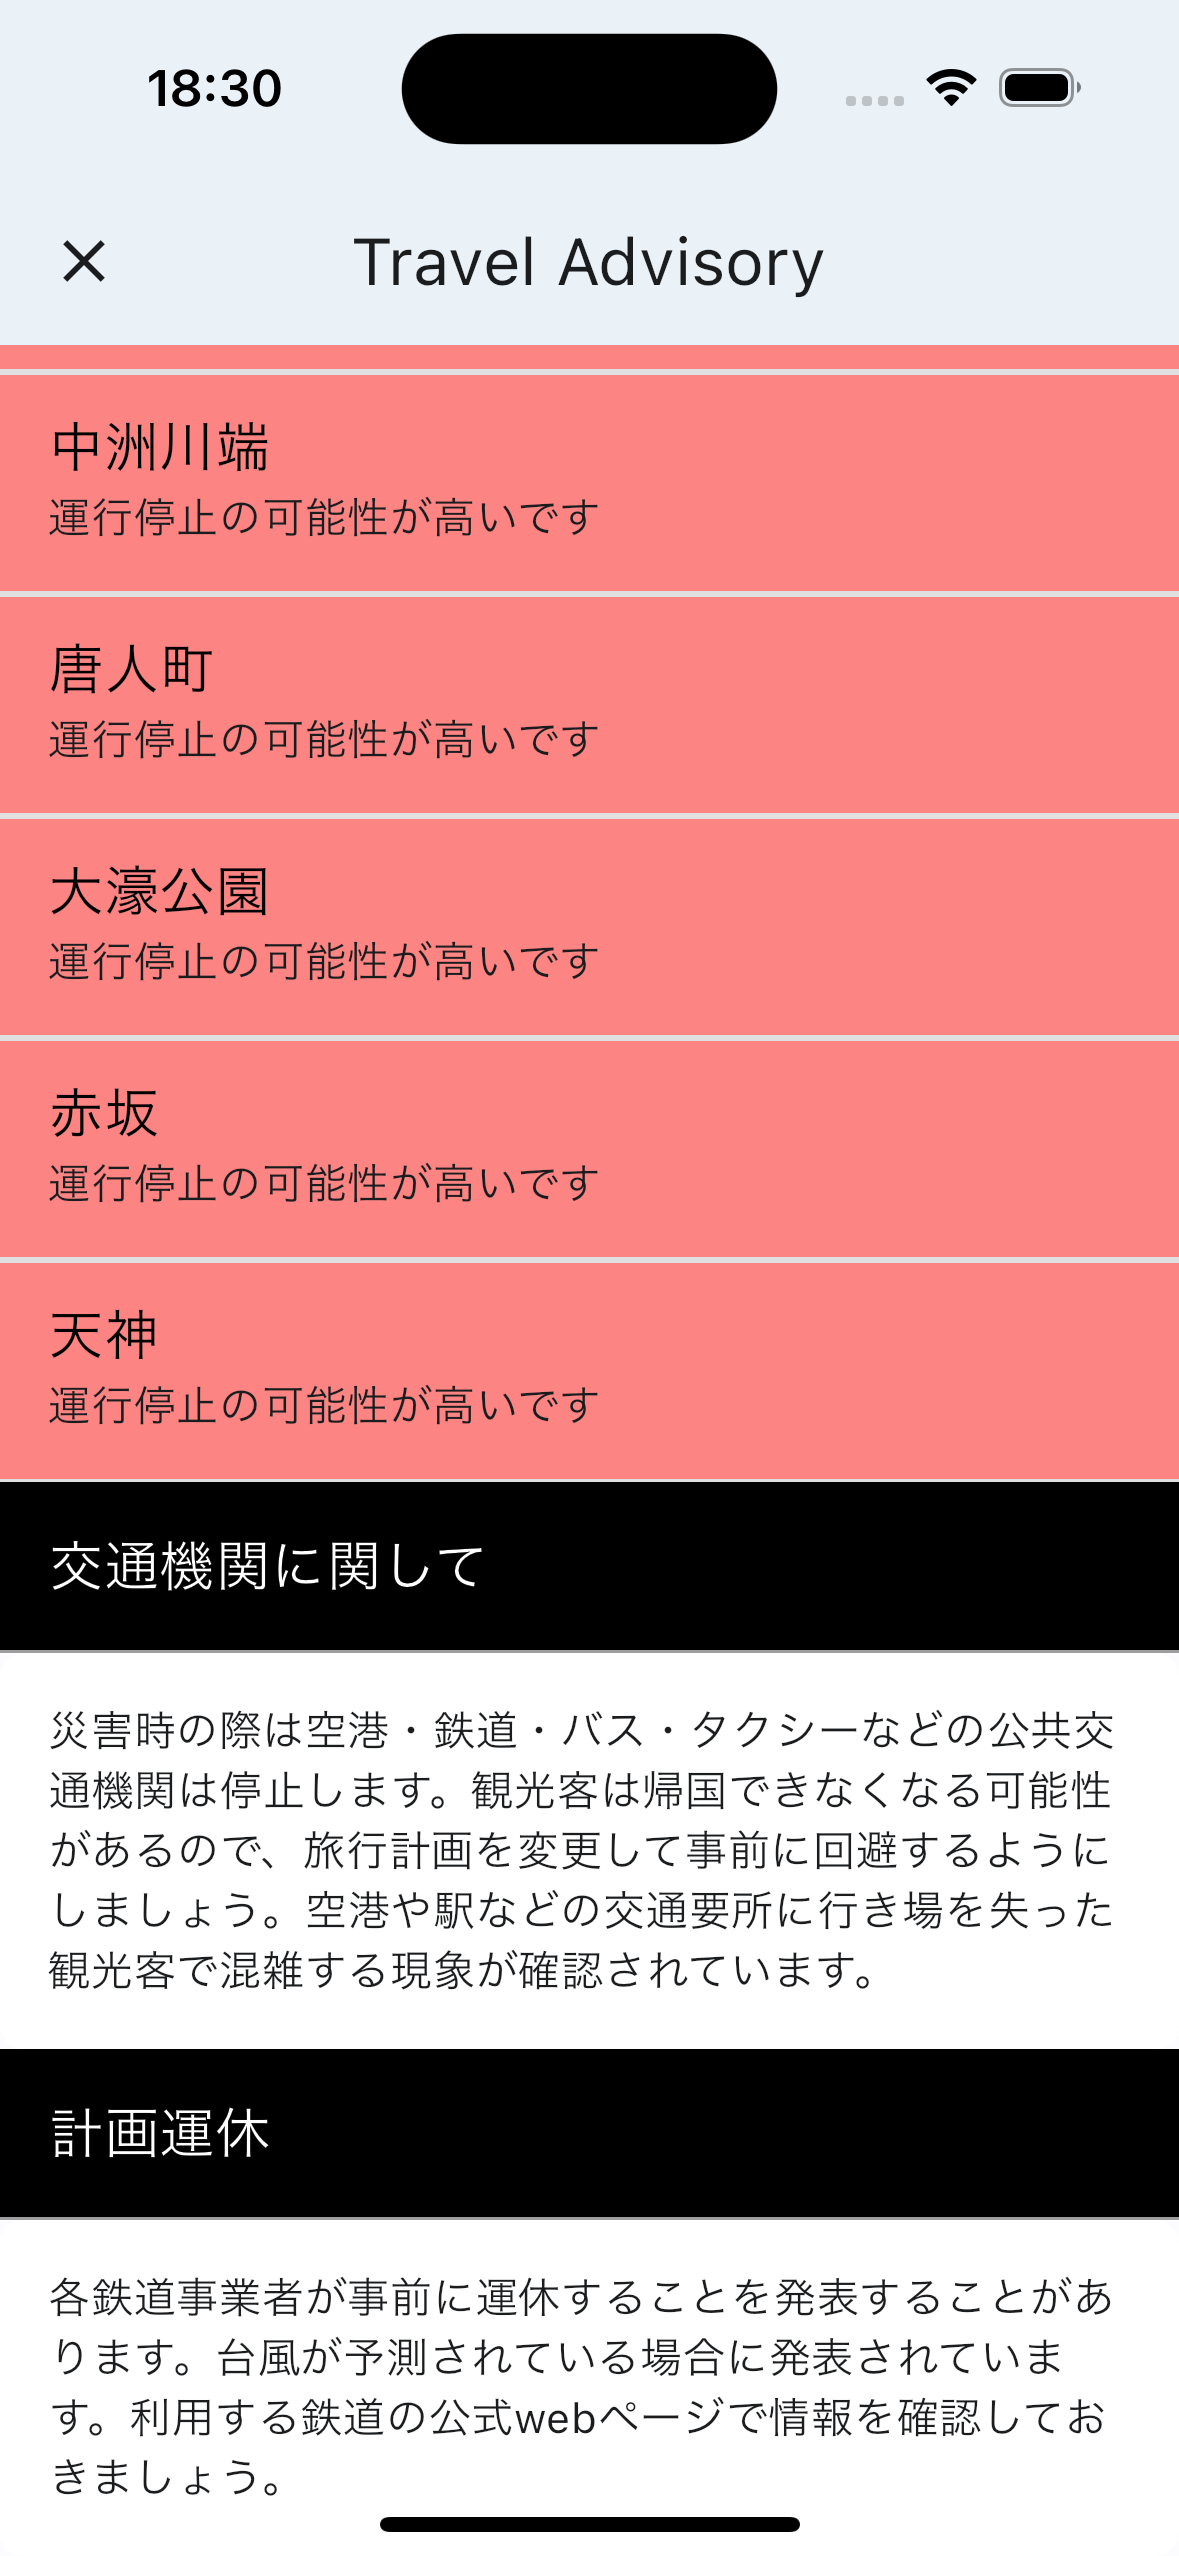
\includegraphics[height=10cm]{./fig/trans_advisory_2.png}
    %\vspace{-3mm}
    \caption{交通データの災害注意予報画面2}
    \label{fig:trans_advisory_2}
    %\vspace{2mm}
  \end{minipage}
\end{figure}

\subsection {ストック情報を確認する}
災害のストック情報を閲覧する.
ストック情報は雨と風(風雪)の2種類の災害の情報である.

\subsubsection {雨の災害の情報}
日本における雨に関する災害についての説明が記載されている.
雨に関する災害とは大雨そのものの現象以外に洪水と土砂災害のことである.
各災害についての説明とそれに対する対策喚起の情報が載っている.

\begin{figure}[H]
  \begin{minipage}[b]{0.45\linewidth}
    \centering
    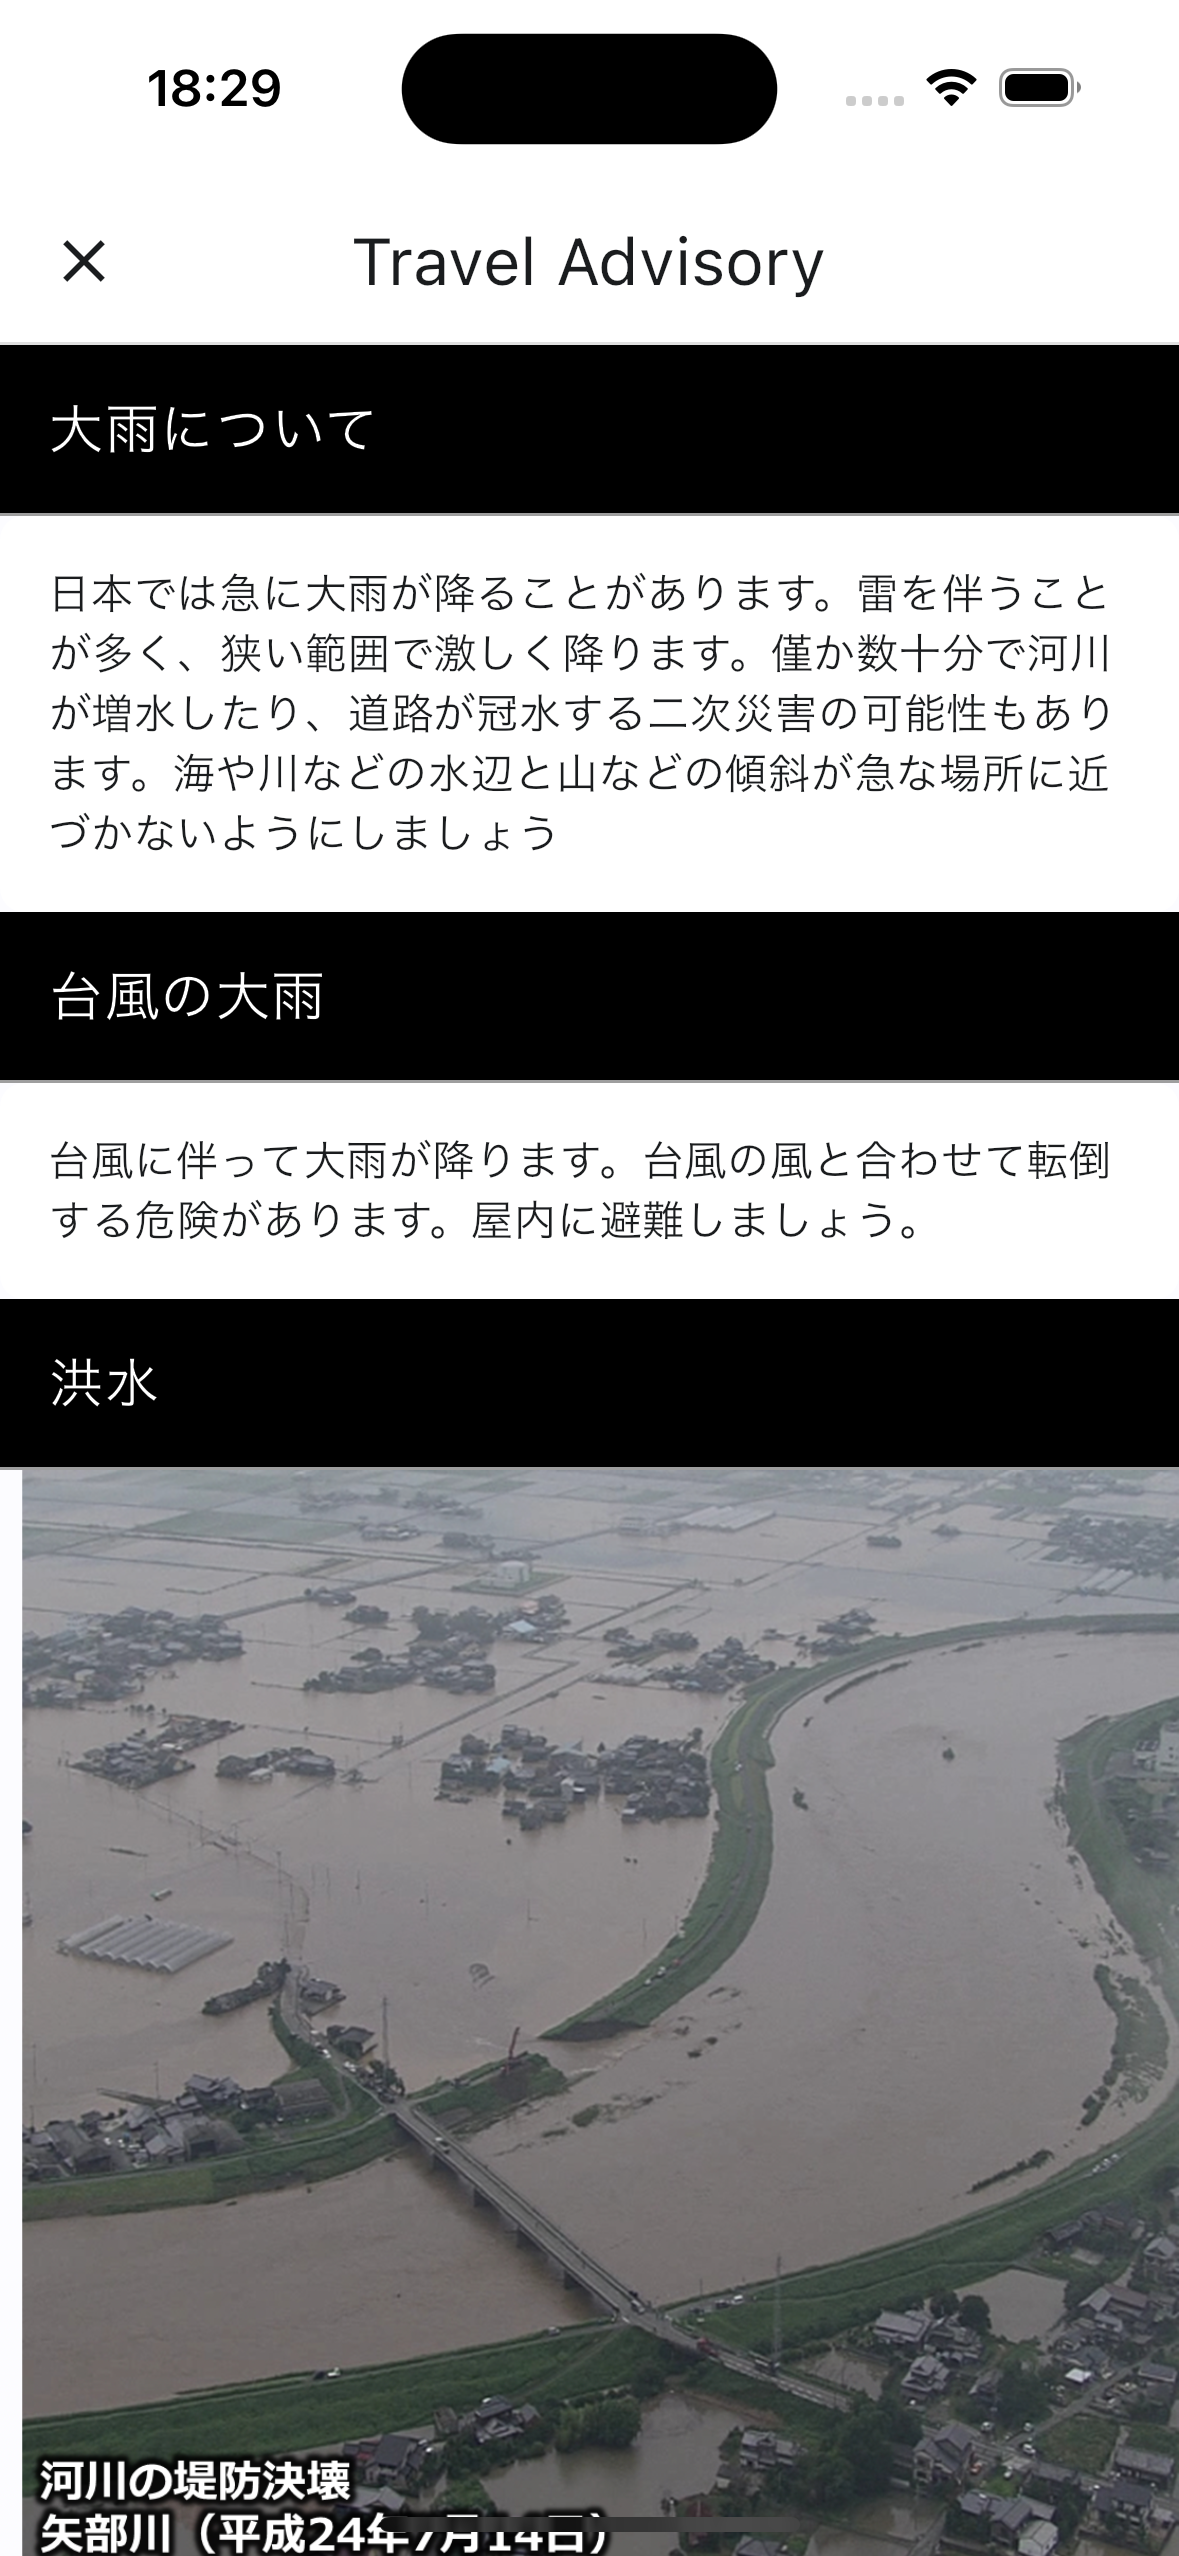
\includegraphics[height=10cm]{./fig/rain_stock_1.png}
    %\vspace{-3mm}
    \caption{雨のストック情報提供画面1}
    \label{fig:rain_stock_1}
    %\vspace{2mm}
  \end{minipage}
  \begin{minipage}[b]{0.45\linewidth}
    \centering
    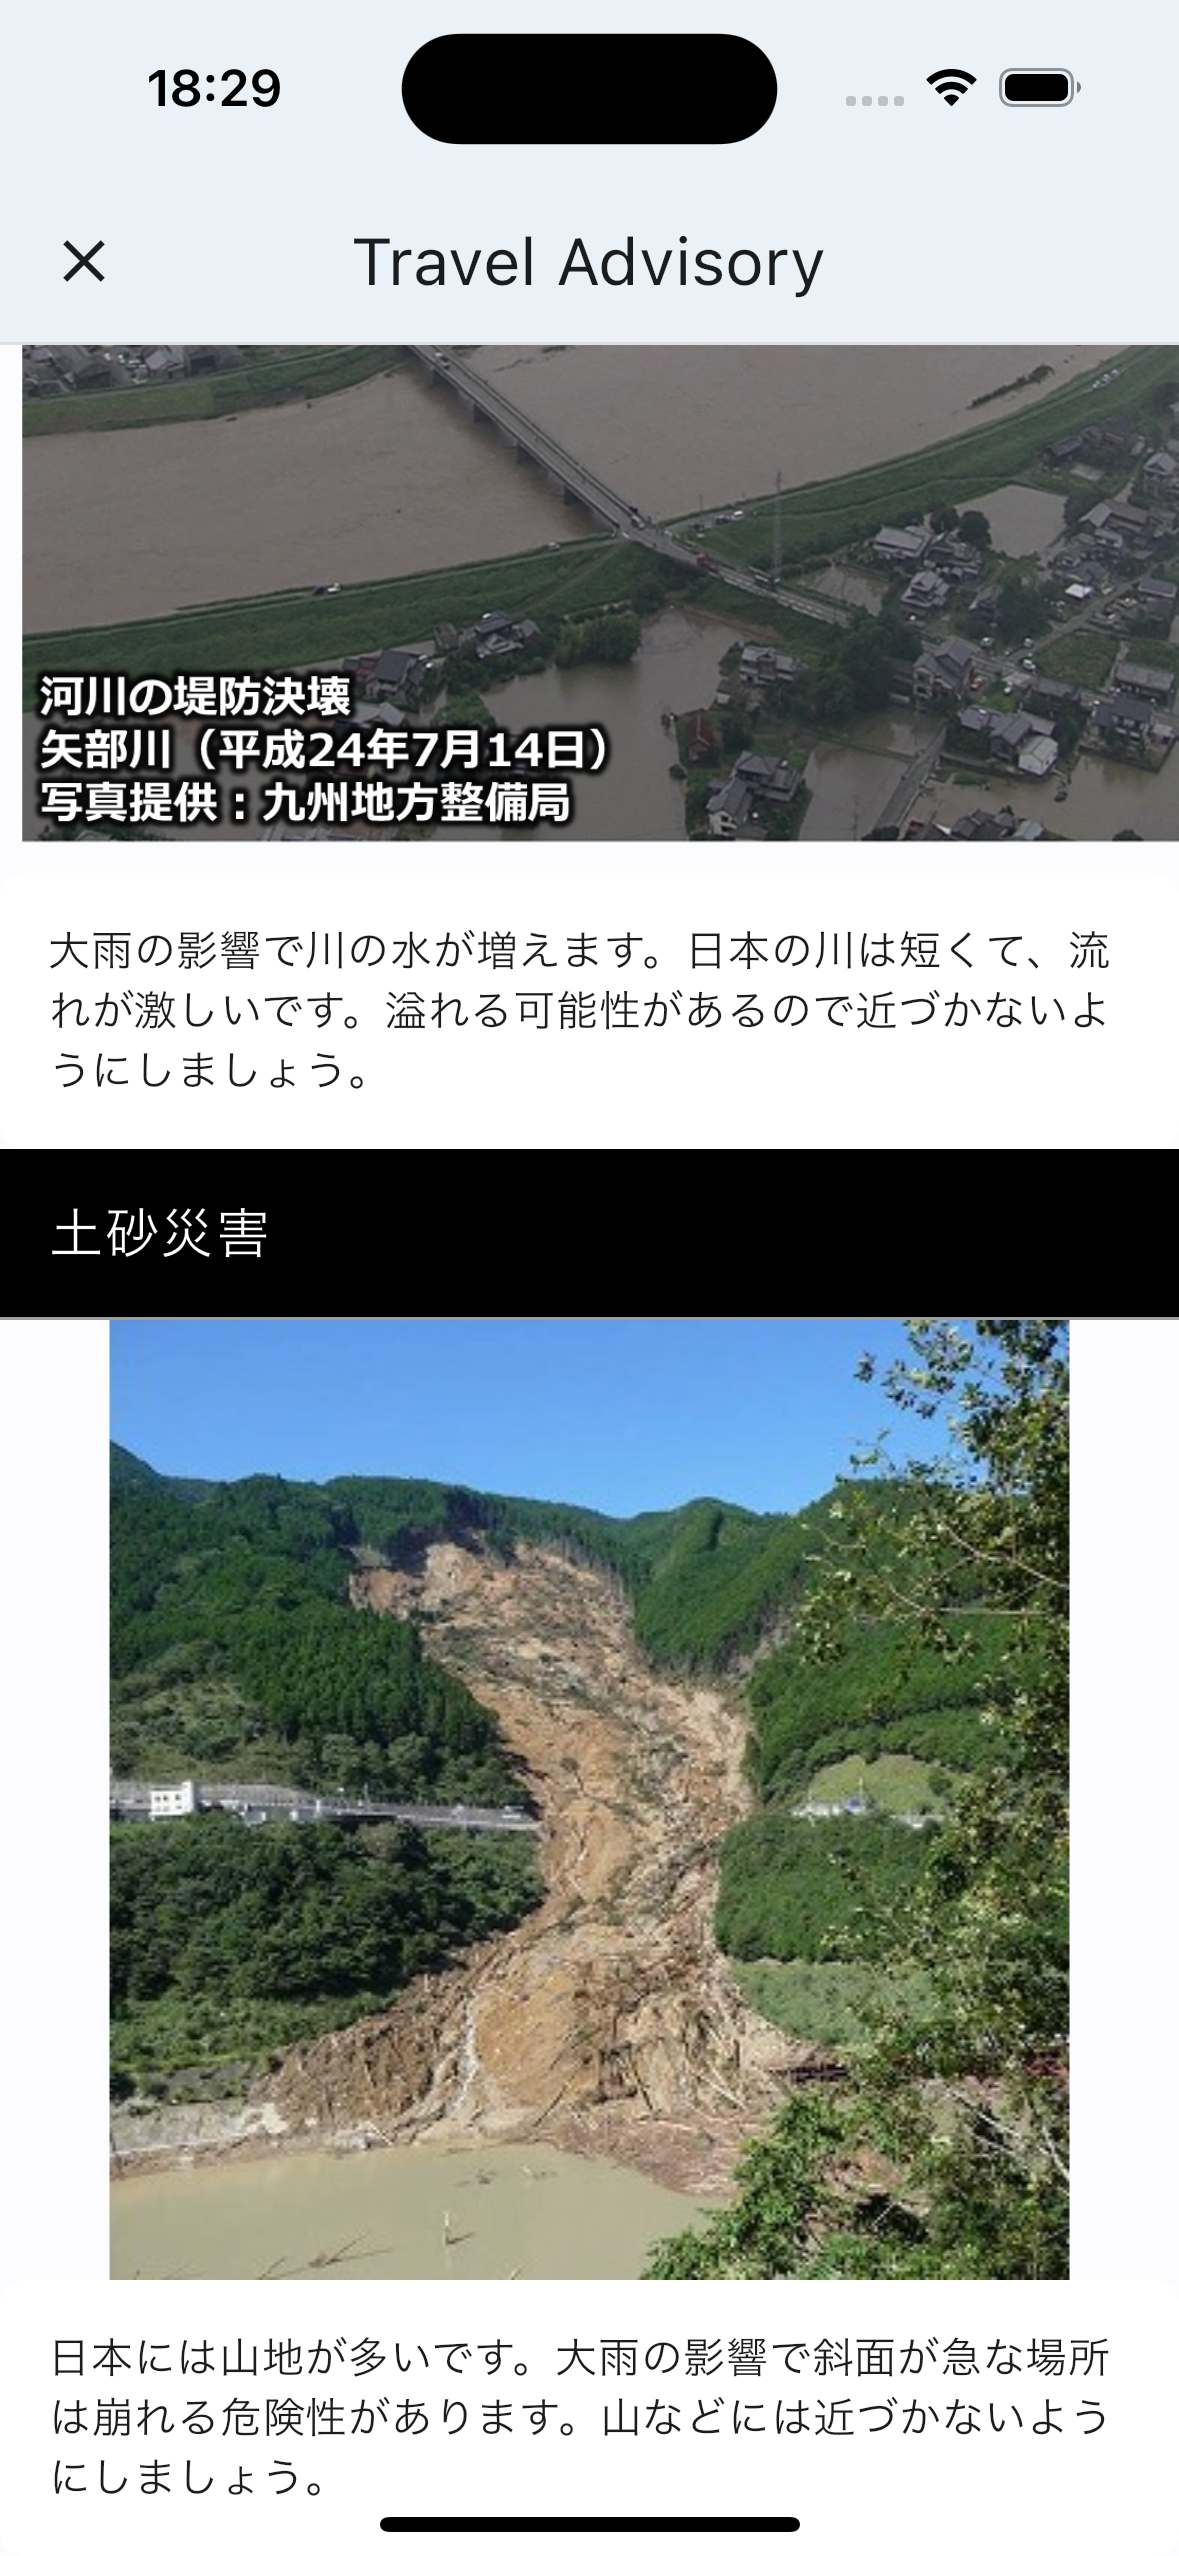
\includegraphics[height=10cm]{./fig/rain_stock_2.png}
    %\vspace{-3mm}
    \caption{雨のストック情報提供画面2}
    \label{fig:rain_stock_2}
    %\vspace{2mm}
  \end{minipage}
\end{figure}

\subsubsection {風の災害の情報}
日本における風に関する災害についての説明が記載されている.
具体的には台風と高潮,暴風についてである.
各災害についての説明とそれに対する対策喚起の情報が載っている.

\begin{figure}[H]
  \begin{minipage}[b]{0.45\linewidth}
    \centering
    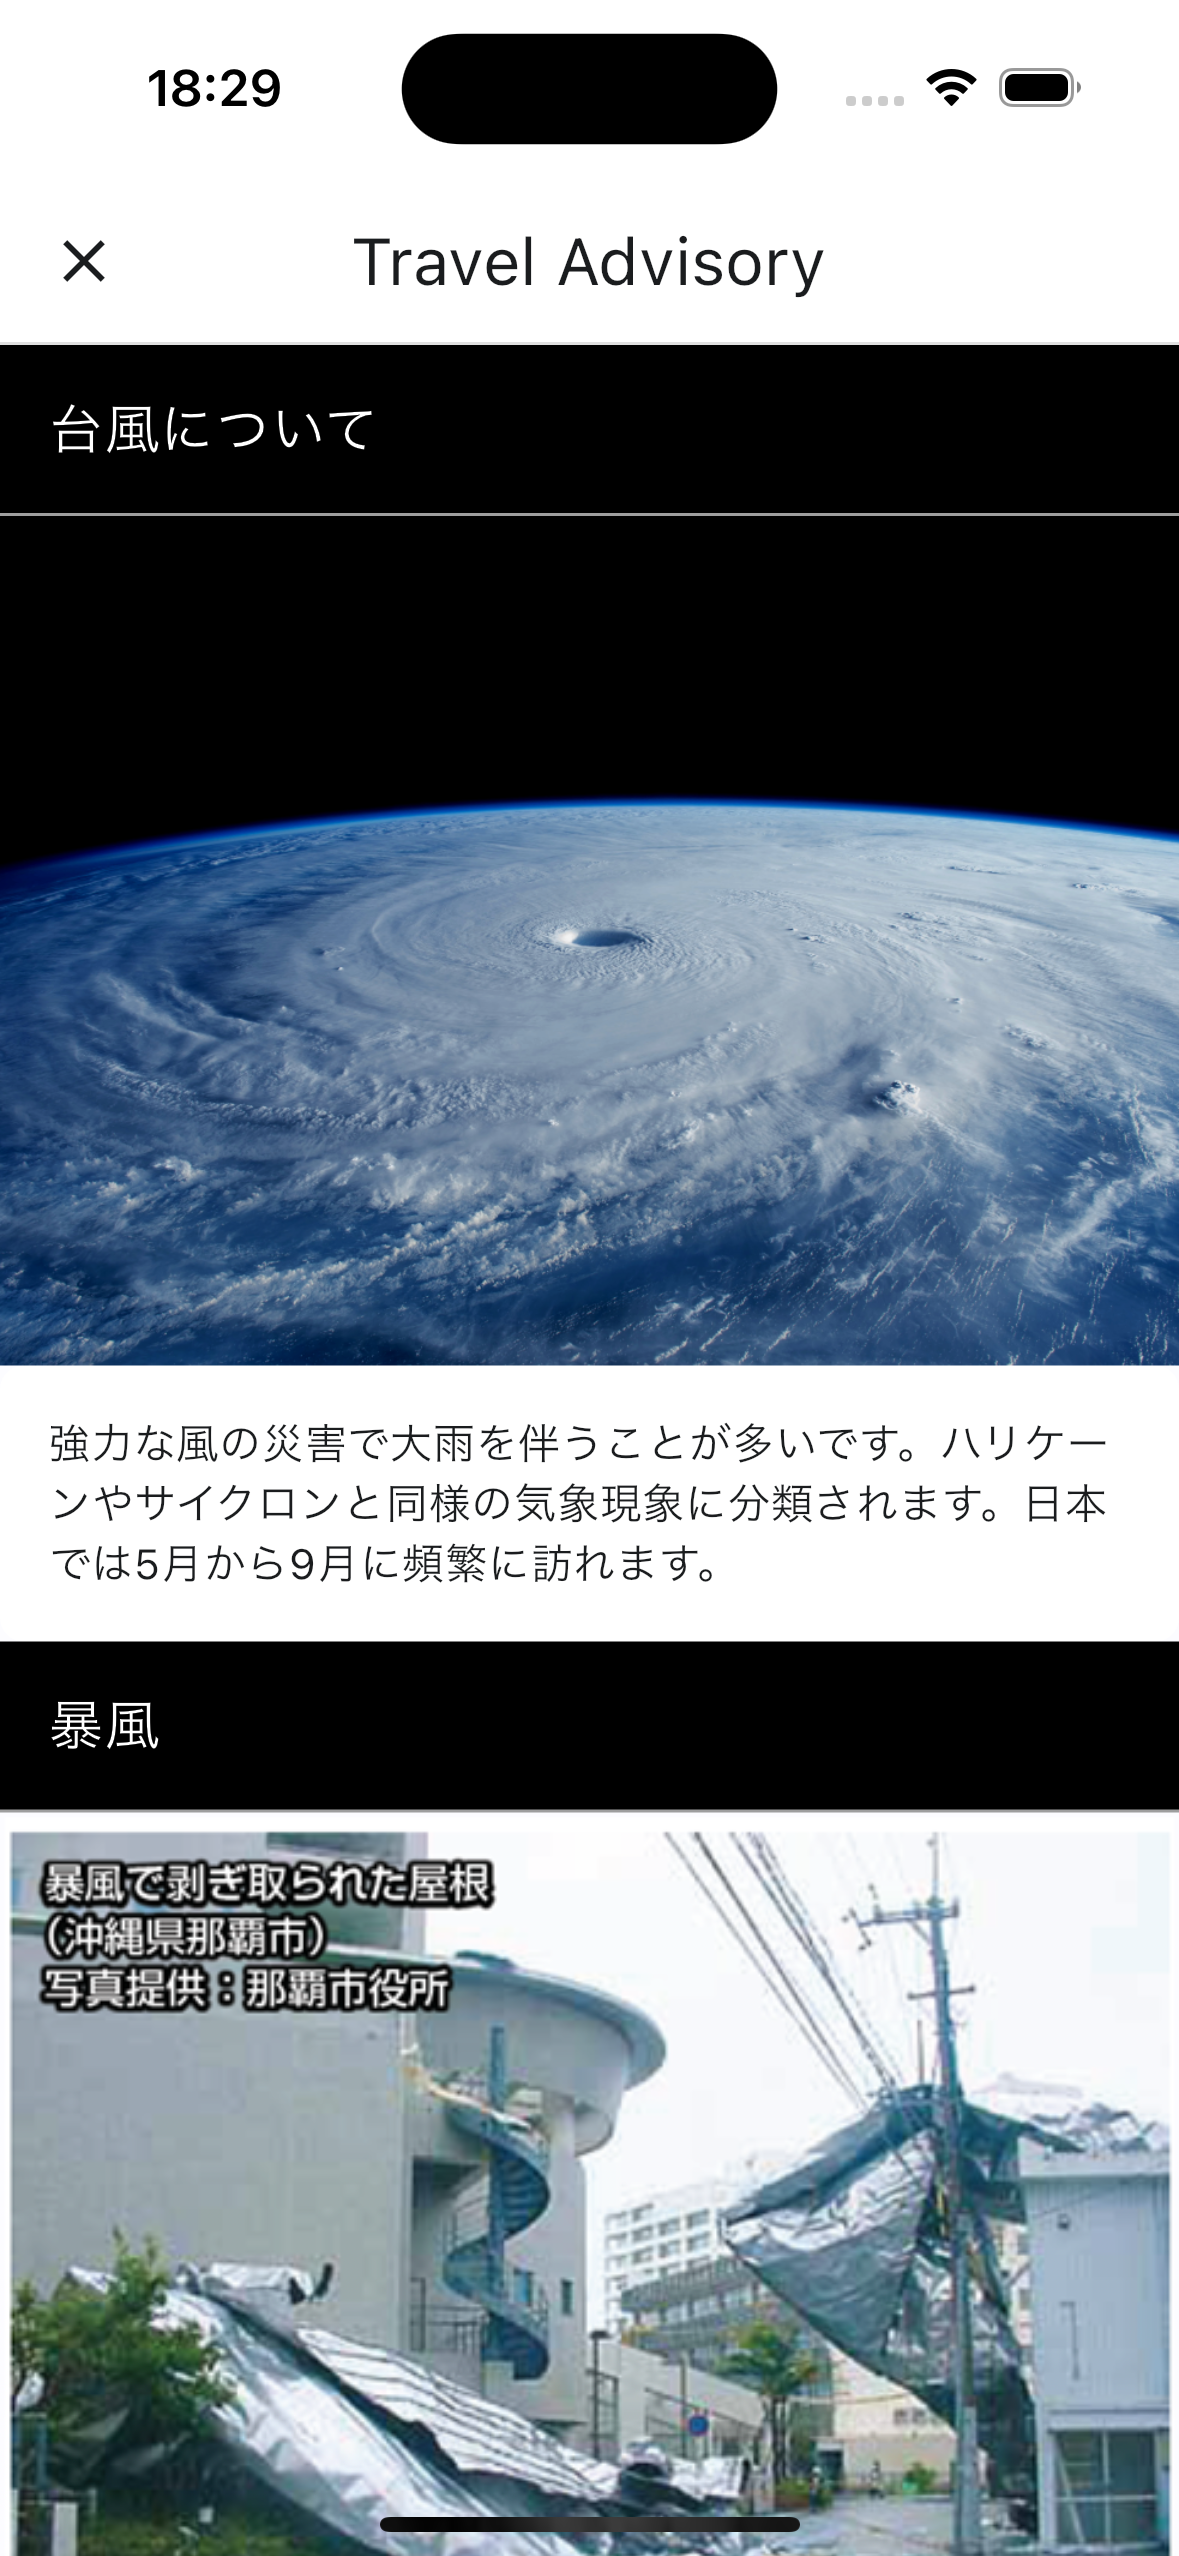
\includegraphics[height=10cm]{./fig/wind_stock_1.png}
    %\vspace{-3mm}
    \caption{風のストック情報提供画面1}
    \label{fig:rain_stock_1}
    %\vspace{2mm}
  \end{minipage}
  \begin{minipage}[b]{0.45\linewidth}
    \centering
    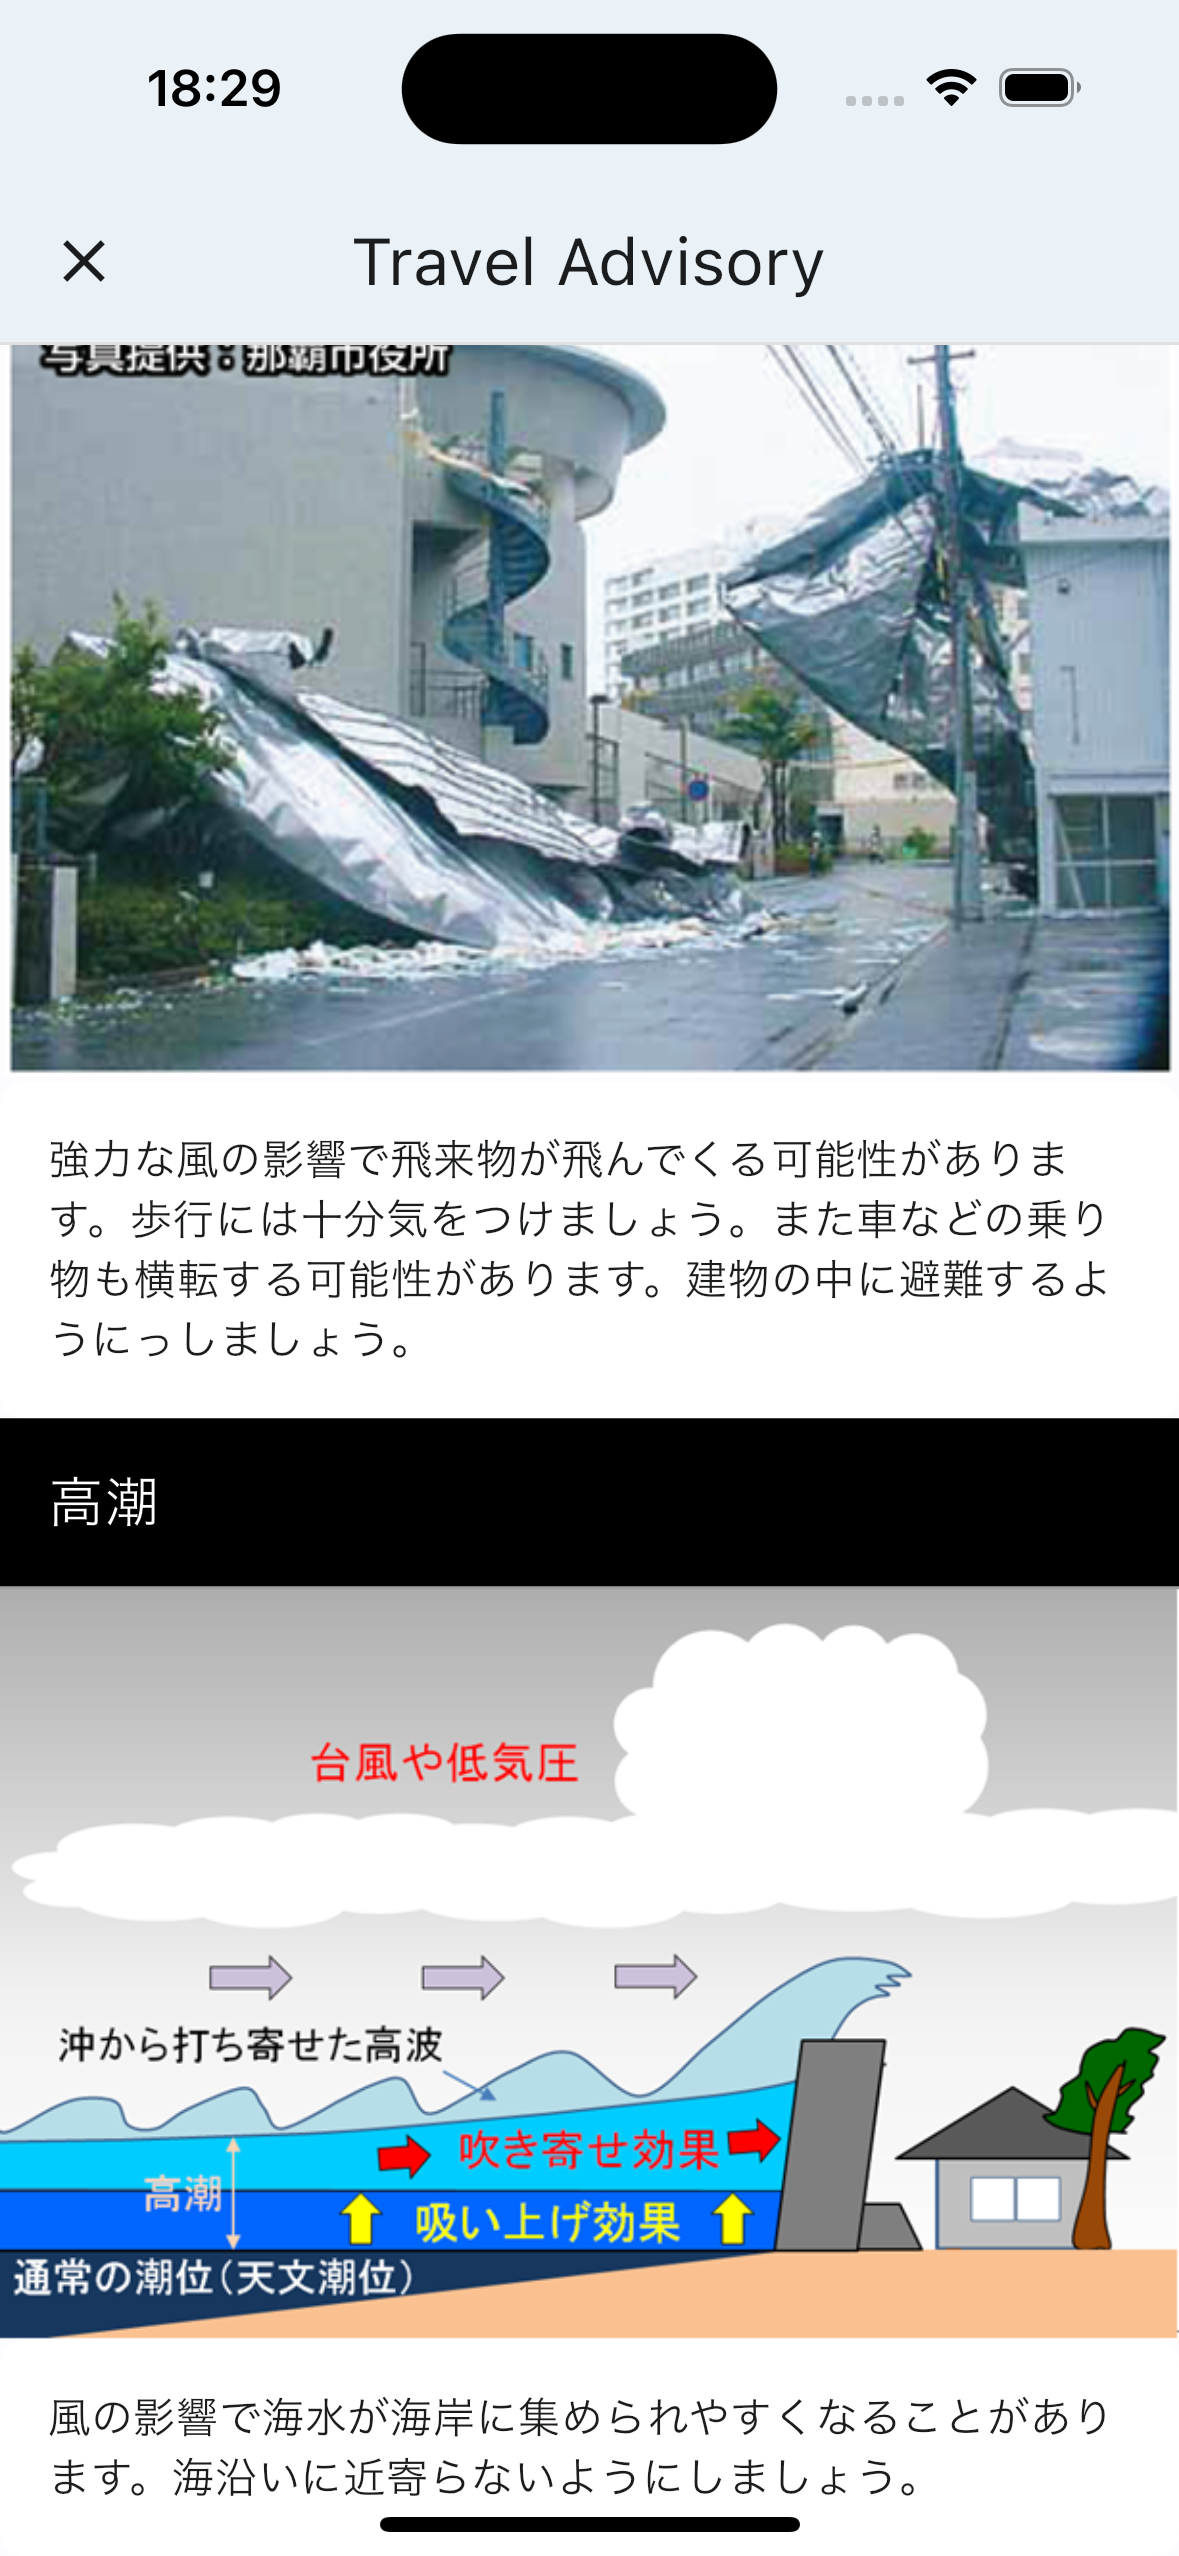
\includegraphics[height=10cm]{./fig/wind_stock_2.png}
    %\vspace{-3mm}
    \caption{風のストック情報提供画面2}
    \label{fig:rain_stock_2}
    %\vspace{2mm}
  \end{minipage}
\end{figure}

% \begin{figure}[H]
%   \centering
%   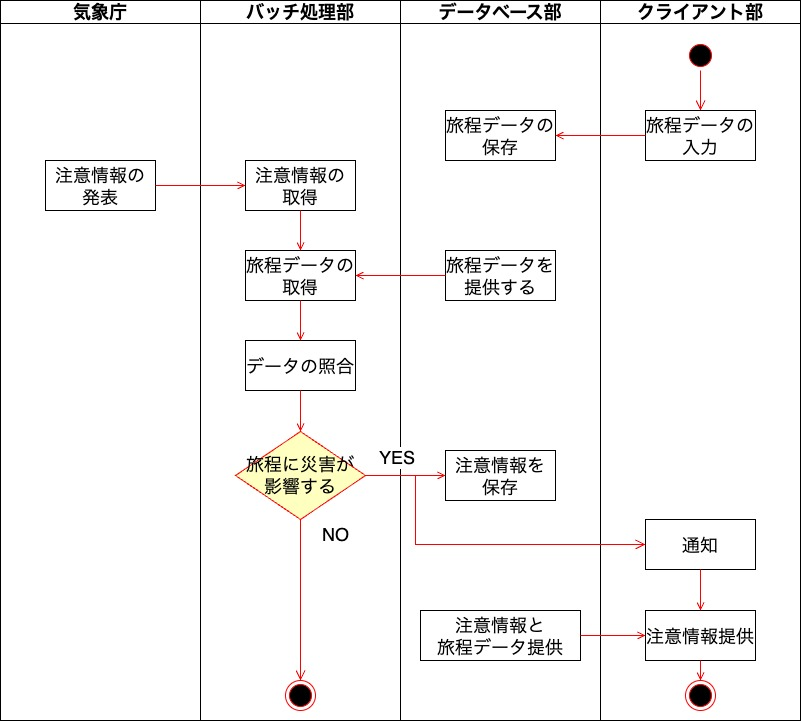
\includegraphics[height=8cm]{figure32.jpg}
%   %\vspace{-3mm}
%   \caption{場所データの注意情報提供画面の図}
%   \label{fig:activity}
%   %\vspace{2mm}
% \end{figure}

% \subsection {公共交通データの注意情報提供画面の図}

% \begin{figure}[H]
%   \centering
%   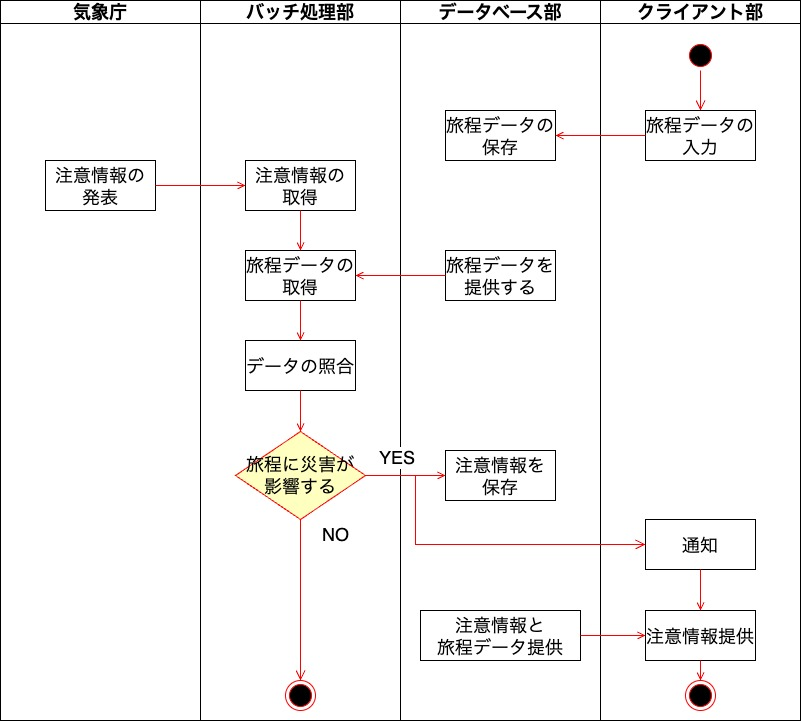
\includegraphics[height=8cm]{figure32.jpg}
%   %\vspace{-3mm}
%   \caption{公共交通データの注意情報提供画面の図}
%   \label{fig:activity}
%   %\vspace{2mm}
% \end{figure}

% \subsection {大雨に関するストック情報の提供画面の図}

% \begin{figure}[H]
%   \centering
%   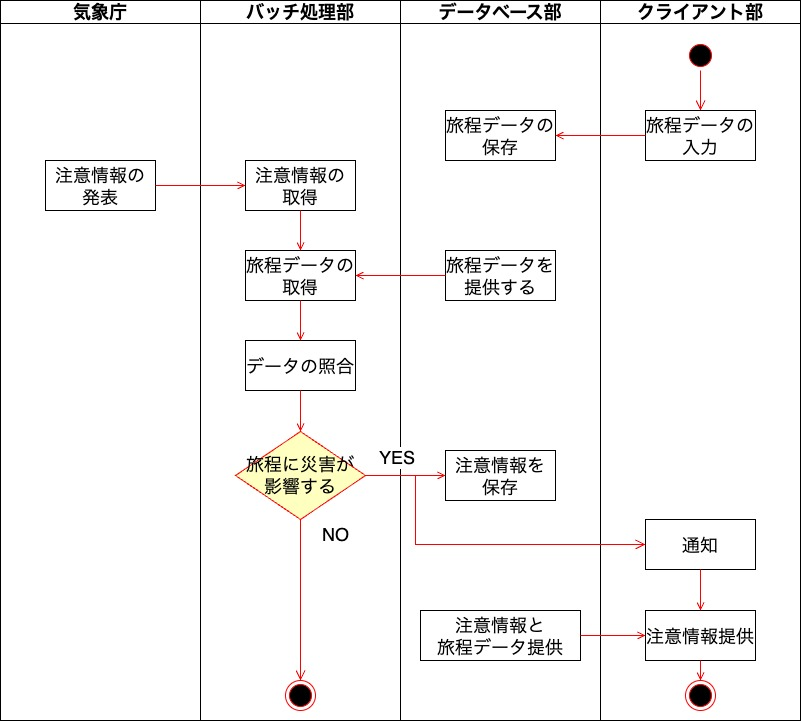
\includegraphics[height=8cm]{figure32.jpg}
%   %\vspace{-3mm}
%   \caption{大雨に関するストック情報の提供画面の図}
%   \label{fig:activity}
%   %\vspace{2mm}
% \end{figure}

% \subsection {風に関するストック情報の提供画面}

% \begin{figure}[H]
%   \centering
%   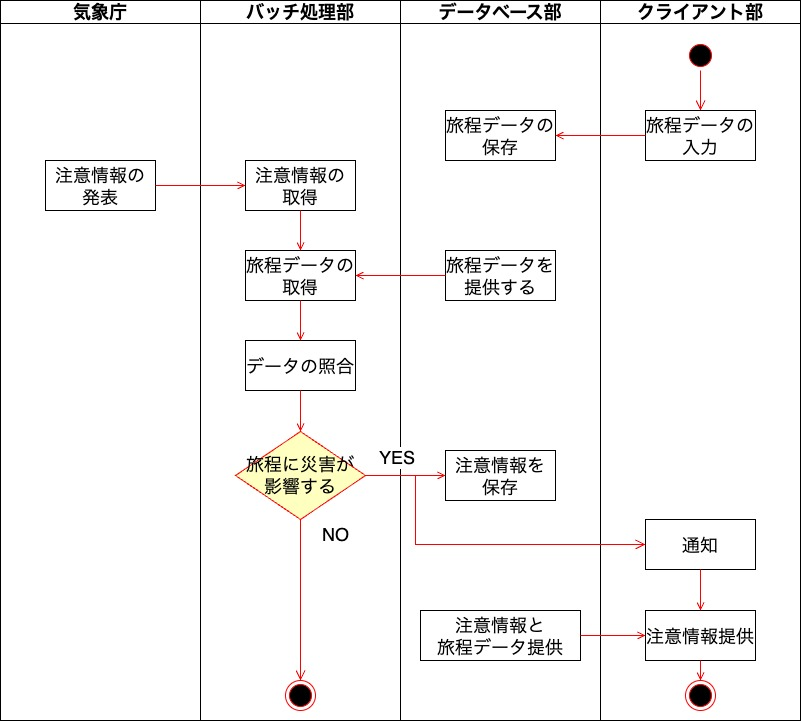
\includegraphics[height=8cm]{figure32.jpg}
%   %\vspace{-3mm}
%   \caption{風に関するストック情報の提供画面の図}
%   \label{fig:activity}
%   %\vspace{2mm}
% \end{figure}